
%\documentclass[3p,times,procedia]{elsarticle}
\documentclass[3p,times,procedia,authoryear,round]{elsarticle}

%% The `ecrc' package must be called to make the CRC functionality available
\usepackage{ecrc}
    \usepackage{float}
    \usepackage{graphicx}
\usepackage{makeidx}  % allows for indexgeneration
\usepackage[english]{babel} % un troisième package
\usepackage{amssymb}
\usepackage{amsmath}
\usepackage{syntax}
\usepackage{multirow}
\usepackage{array}
\usepackage[table]{xcolor}
\usepackage{enumitem}
\usepackage{booktabs}
\usepackage{listings}
%\usepackage{caption}
\usepackage{subcaption}
\usepackage{courier}
\usepackage{mathrsfs}
%\usepackage[authoryear]{natbib}
\usepackage{amsthm}

\usepackage{subcaption}
%\usepackage[]{algorithm2e}
\usepackage{algorithm}
%\usepackage{algorithmic}
\usepackage{algpseudocode}
\usepackage{hyperref}
\hypersetup{
  colorlinks,
  citecolor= 	JungleGreen,
  linkcolor= 	JungleGreen,
  urlcolor= 	JungleGreen}
\usepackage{rotating}
\usepackage[T1]{fontenc}
\usepackage[utf8]{inputenc}
\usepackage{amsmath,amsfonts,amssymb}
%\hypersetup{colorlinks=true,citecolor=blue}% just for the example
%% The ecrc package defines commands needed for running heads and logos.
%% For running heads, you can set the journal name, the volume, the starting page and the authors
%\RequirePackage[authoryear]{natbib}
%\usepackage[authoryear,round]{natbib}
%\bibpunct{(}{)}{,}{a}{,}{,}
%% set the volume if you know. Otherwise `00'
%\biboptions{authoryear,round}

\volume{00}

%% set the starting page if not 1
\firstpage{1}

%% Give the name of the journal
\journalname{Information \& Software Technology}

%% Give the author list to appear in the running head
%% Example \runauth{C.V. Radhakrishnan et al.}
\runauth{}
%% Give the abbreviation of the Journal.  Contact the journal editorial office if in any doubt
\jid{procs}

%% Give a short journal name for the dummy logo (if needed)
\jnltitlelogo{ \small Information \& Software Technology}
\normalsize
%% Provide the copyright line to appear in the abstract
%% Usage:
%   \CopyrightLine[<text-before-year>]{<year>}{<restt-of-the-copyright-text>}
%   \CopyrightLine[Crown copyright]{2011}{Published by Elsevier Ltd.}
%   \CopyrightLine{2011}{Elsevier Ltd. All rights reserved}
%\CopyrightLine{2014}{Published by Elsevier Ltd.}

%% Hereafter the template follows `elsarticle'.
%% For more details see the existing template files elsarticle-template-harv.tex and elsarticle-template-num.tex.

%% Elsevier CRC generally uses a numbered reference style
%% For this, the conventions of elsarticle-template-num.tex should be followed (included below)
%% If using BibTeX, use the style file elsarticle-num.bst

%% End of ecrc-specific commands
%%%%%%%%%%%%%%%%%%%%%%%%%%%%%%%%%%%%%%%%%%%%%%%%%%%%%%%%%%%%%%%%%%%%%%%%%%

%% The amssymb package provides various useful mathematical symbols
\usepackage{amssymb}
%% The amsthm package provides extended theorem environments
%% \usepackage{amsthm}

%% The lineno packages adds line numbers. Start line numbering with
%% \begin{linenumbers}, end it with \end{linenumbers}. Or switch it on
%% for the whole article with \linenumbers after \end{frontmatter}.
%% \usepackage{lineno}

%% natbib.sty is loaded by default. However, natbib options can be
%% provided with \biboptions{...} command. Following options are
%% valid:

%%   round  -  round parentheses are used (default)
%%   square -  square brackets are used   [option]
%%   curly  -  curly braces are used      {option}
%%   angle  -  angle brackets are used    <option>
%%   semicolon  -  multiple citations separated by semi-colon
%%   colon  - same as semicolon, an earlier confusion
%%   comma  -  separated by comma
%%   numbers-  selects numerical citations
%%   super  -  numerical citations as superscripts
%%   sort   -  sorts multiple citations according to order in ref. list
%%   sort&compress   -  like sort, but also compresses numerical citations
%%   compress - compresses without sorting
%%
%% \biboptions{comma,round}

% \biboptions{}

% if you have landscape tables

% put your own definitions here:
%   \newcommand{\cZ}{\cal{Z}}
%   \newtheorem{def}{Definition}[section]
%   ...

% add words to TeX's hyphenation exception list
%\hyphenation{author another created financial paper re-commend-ed Post-Script}

% declarations for front matter
\usepackage{enumitem}
\begin{document}

\begin{frontmatter}

%% Title, authors and addresses

%% use the tnoteref command within \title for footnotes;
%% use the tnotetext command for the associated footnote;
%% use the fnref command within \author or \address for footnotes;
%% use the fntext command for the associated footnote;
%% use the corref command within \author for corresponding author footnotes;
%% use the cortext command for the associated footnote;
%% use the ead command for the email address,
%% and the form \ead[url] for the home page:
%%
%% \title{Title\tnoteref{label1}}
%% \tnotetext[label1]{}
%% \author{Name\corref{cor1}\fnref{label2}}
%% \ead{email address}
%% \ead[url]{home page}
%% \fntext[label2]{}
%% \cortext[cor1]{}
%% \address{Address\fnref{label3}}
%% \fntext[label3]{}

\dochead{}
%% Use \dochead if there is an article header, e.g. \dochead{Short communication}
%% \dochead can also be used to include a conference title, if directed by the editors
%% e.g. \dochead{17th International Conference on Dynamical Processes in Excited States of Solids}

\title{
Reliability analysis based on probabilistic model checking for software deployment in embedded systems}

%% use optional labels to link authors explicitly to addresses:
%% \author[label1,label2]{<author name>}
%% \address[label1]{<address>}
%% \address[label2]{<address>}
\author[aut1]{Abdelhakim Baouya\corref{cor1}}
\ead{baouya.abdelhakim@gmail.com}
\author[aut2]{Djamal Bennouar}
\ead{dbennouar@gmail.com}
\author[aut3]{Otmane Ait Mohamed}
\ead{otmane.aitmohamed@concordia.ca}
\author[aut4]{Samir Ouchani}
\ead{samir\_ouchani@yahoo.com}
%% The choice of journal logo is determined by the \jid and \jnltitlelogo commands.
%% A user-supplied logo with the name <\jid>logo.pdf will be inserted if present.
%% e.g. if \jid{yspmi} the system will look for a file yspmilogo.pdf
%% Otherwise the content of \jnltitlelogo will be set between horizontal lines as a default logo
\cortext[cor1]{Corresponding author at : CS Department, University of BLIDA 1, Blida, Algeria. Tel.:+213 794 005 852 }

\address[aut1]{University of BLIDA 1 , Blida , Algeria, LIMPAF \& LRDSI Lab, CS Department}
\address[aut2]{University of Bouira, Algeria, LIMPAF Lab, CS Department}
\address[aut3]{Concordia University, Montr\'{e}al, Canada, ECE Department}
\address[aut4]{University of Luxembourg, Luxembourg, SnT Center}
%\author{}

%\address{}

\begin{abstract}
    
%\begin{description}
   %[align=left]
    
    \noindent
\emph{Context}: Todays, embedded systems span a wide range from a small platform of sensors and actuators to a distributed systems combining a huge number of interacting nodes. Designing such systems includes hardware parts and software parts. Software parts gain more and more importance since  it handles the complex embedded system functionality.  The deployment of software components to hardware nodes is very hard and time-consuming to determine whether its design fulfills the reliability requirements.


 \noindent
\emph{Objective}: To efficiently exploit the physical platform in the software development process, we introduce a novel approach in deployment-decision making based on PRISM probabilistic model checker that takes the software components and the physical platform to produce a set of deployment candidates. 


 \noindent
\emph{Method}: We construct our framework on System Modeling Language (SysML). The framework includes mechanisms to extract hardware and software properties and to produce the deployment candidates.  To check the best one, each candidate should satisfy the reliability property that is expressed in Probabilistic Computation Tree Logic. 


 \noindent
\emph{Results}:  We capture the underlying semantics of the software blocks behavior expressed as an activity diagram and their generated PRISM code to prove the soundness of the approach. We found that the probabilistic equivalence relation between both semantics preserves the satisfaction of the system requirements. We present the automotive control system as case study to illustrate the applicability of the proposed approach.     


 \noindent
 \emph{Conclusion}: Our methodology provide designers with optimal deployment candidate based on the reliability attributes. This solution based on SysML and probabilistic model checking is implemented as a software tool. 
 
 
%\end{description}      
\end{abstract}

\begin{keyword}
SysML internal block  diagrams\sep  Activity diagrams\sep Reliability\sep  Model checking\sep Deployment
%% keywords here, in the form: keyword \sep keyword

%% PACS codes here, in the form: \PACS code \sep code

%% MSC codes here, in the form: \MSC code \sep code
%% or \MSC[2008] code \sep code (2000 is the default)

\end{keyword}

\end{frontmatter}

%%
%% Start line numbering here if you want
%%
% \linenumbers

%% main text
\section{Introduction}
\label{Introduction}

Many cities are more and more overcrowded and lead to the growing accidents and unpredicted emergencies. In response to that, the engineers have to open a way to improve the safety and efficiency. Several innovative and cost-effective solutions are emerging to simplify our daily-life so-called Automotive Control Systems (ACS) \citep{Reif2014}. The evolution of \emph{ Automotive Control Systems} is enabled by recent advances in computing and sensing technologies as well as advances in estimation and control theory. However, restrictions on such systems in terms of reliability, safety, security are becoming more stringent. In one side these systems are increasingly complex, in the other side the hardware platform resources are often limited in memory, number of hardware interfaces, communication bandwidth, and so on, which make the task of its design hard. One major challenge in this process is to enhance the system reliability by taking in account the restricted physical resources as well as their failure. \citep{Rashid6933951} assert that the hardware faults have a negative impacts on the programs (i.e. software). So, considering these assertions, the high-level description will provide sufficient information to predict system reliability in our deployment plan.

Software deployment is a complex procedure known to be NP-hard \citep{Garey1979}, the process consists in the distribution of a software components on different physical locations with respect to the requirements. The term \emph{component} refers to an operational unit or modules consisting in set of operations where the assembled components represent a system. Note that the component-based development approach is a proven concept for managing complexity \citep{Carlson2006127}, and it has been used also in embedded system design for a while \citep{Herrera201455}. In case of software-hardware deployment, we have to distinguish two set of components; hardware and software communicating using a proper interface. \citep{Arcangeli2015198} and \citep{5934806} give a state of the art related to the deployment concepts and existed strategies.  

Reliability is one of the quality attributes for the achievement of the deployment with minimum failures. This issue is addressed by \citep{Baouya2016} in order to increase reliability and to plan maintenance strategies of multi-processing systems. In our approach, we want to optimize the deployment with respect to system reliability computed from a set of quality attributes.  Numerous publications such as \citep{Zhang2013261}, \citep{Peng2014}, \citep{Lu201595} and \citep{Cherfi201442} discussed about reliability and state that the methods rely on the application of Markov models. One of the interesting approach is Probabilistic model checking \citep{Kwiatkowska},  a quantitative analysis technique based on Markov models.  It has been proven its usefulness in case of analyzing a wide range of reliability and availability properties \citep{Zhang2013261} \citep{Hoque2014}. 


In our study, we mainly deal with  this kind of relationship between the software blocks and executing platform represented by processors and buses, and we study the architectural alternatives that could take our system by the deployment of software components on the processors. For this purpose, we specify our electronic system using SysML diagrams \citep{OMG} and the satisfaction of our properties depends on the behavior of its core software. 


The basic idea is to first build a  parameterizable Markov model \citep{Filieri2016} that captures the software behavior expressed in SysML activity diagrams, and then to check the property on the model using temporal logic. The input parameters represent the reliability computed from the properties of our electronic automotive system and the results of the software-hardware allocations. In order to allow for automatic verification using PRISM \citep{Kwiatkowska}, the underlying \emph{Discrete-time Markov Chains} (DTMC) semantic model of system behavior is constructed using the semantic rules. DTMC is used under the assumption that the system’s behavior meets with some tolerable approximation of the Markov property, i.e. the probability of moving to the next state  depends only on the current state, not on the history that lead to that state \citep{KP12}.  Fig.\ref{approach} depicts all the steps for the deployment-space exploration (DSE). The specification consists on the SysML Internal Block Diagram (IBD) of both software and hardware components with its behavior expressed in activity diagrams. The instances of blocks called \emph{parts} are enriched with MARTE features (Modeling and Analysis of Real-Time and Embedded systems) \citep{Mallet} to express software and hardware characteristics such as workloads. To illustrate the use of transformations in this process, we study the deployment of sub parts of automotive control system. 

\begin{figure}[!ht]
	\centering
	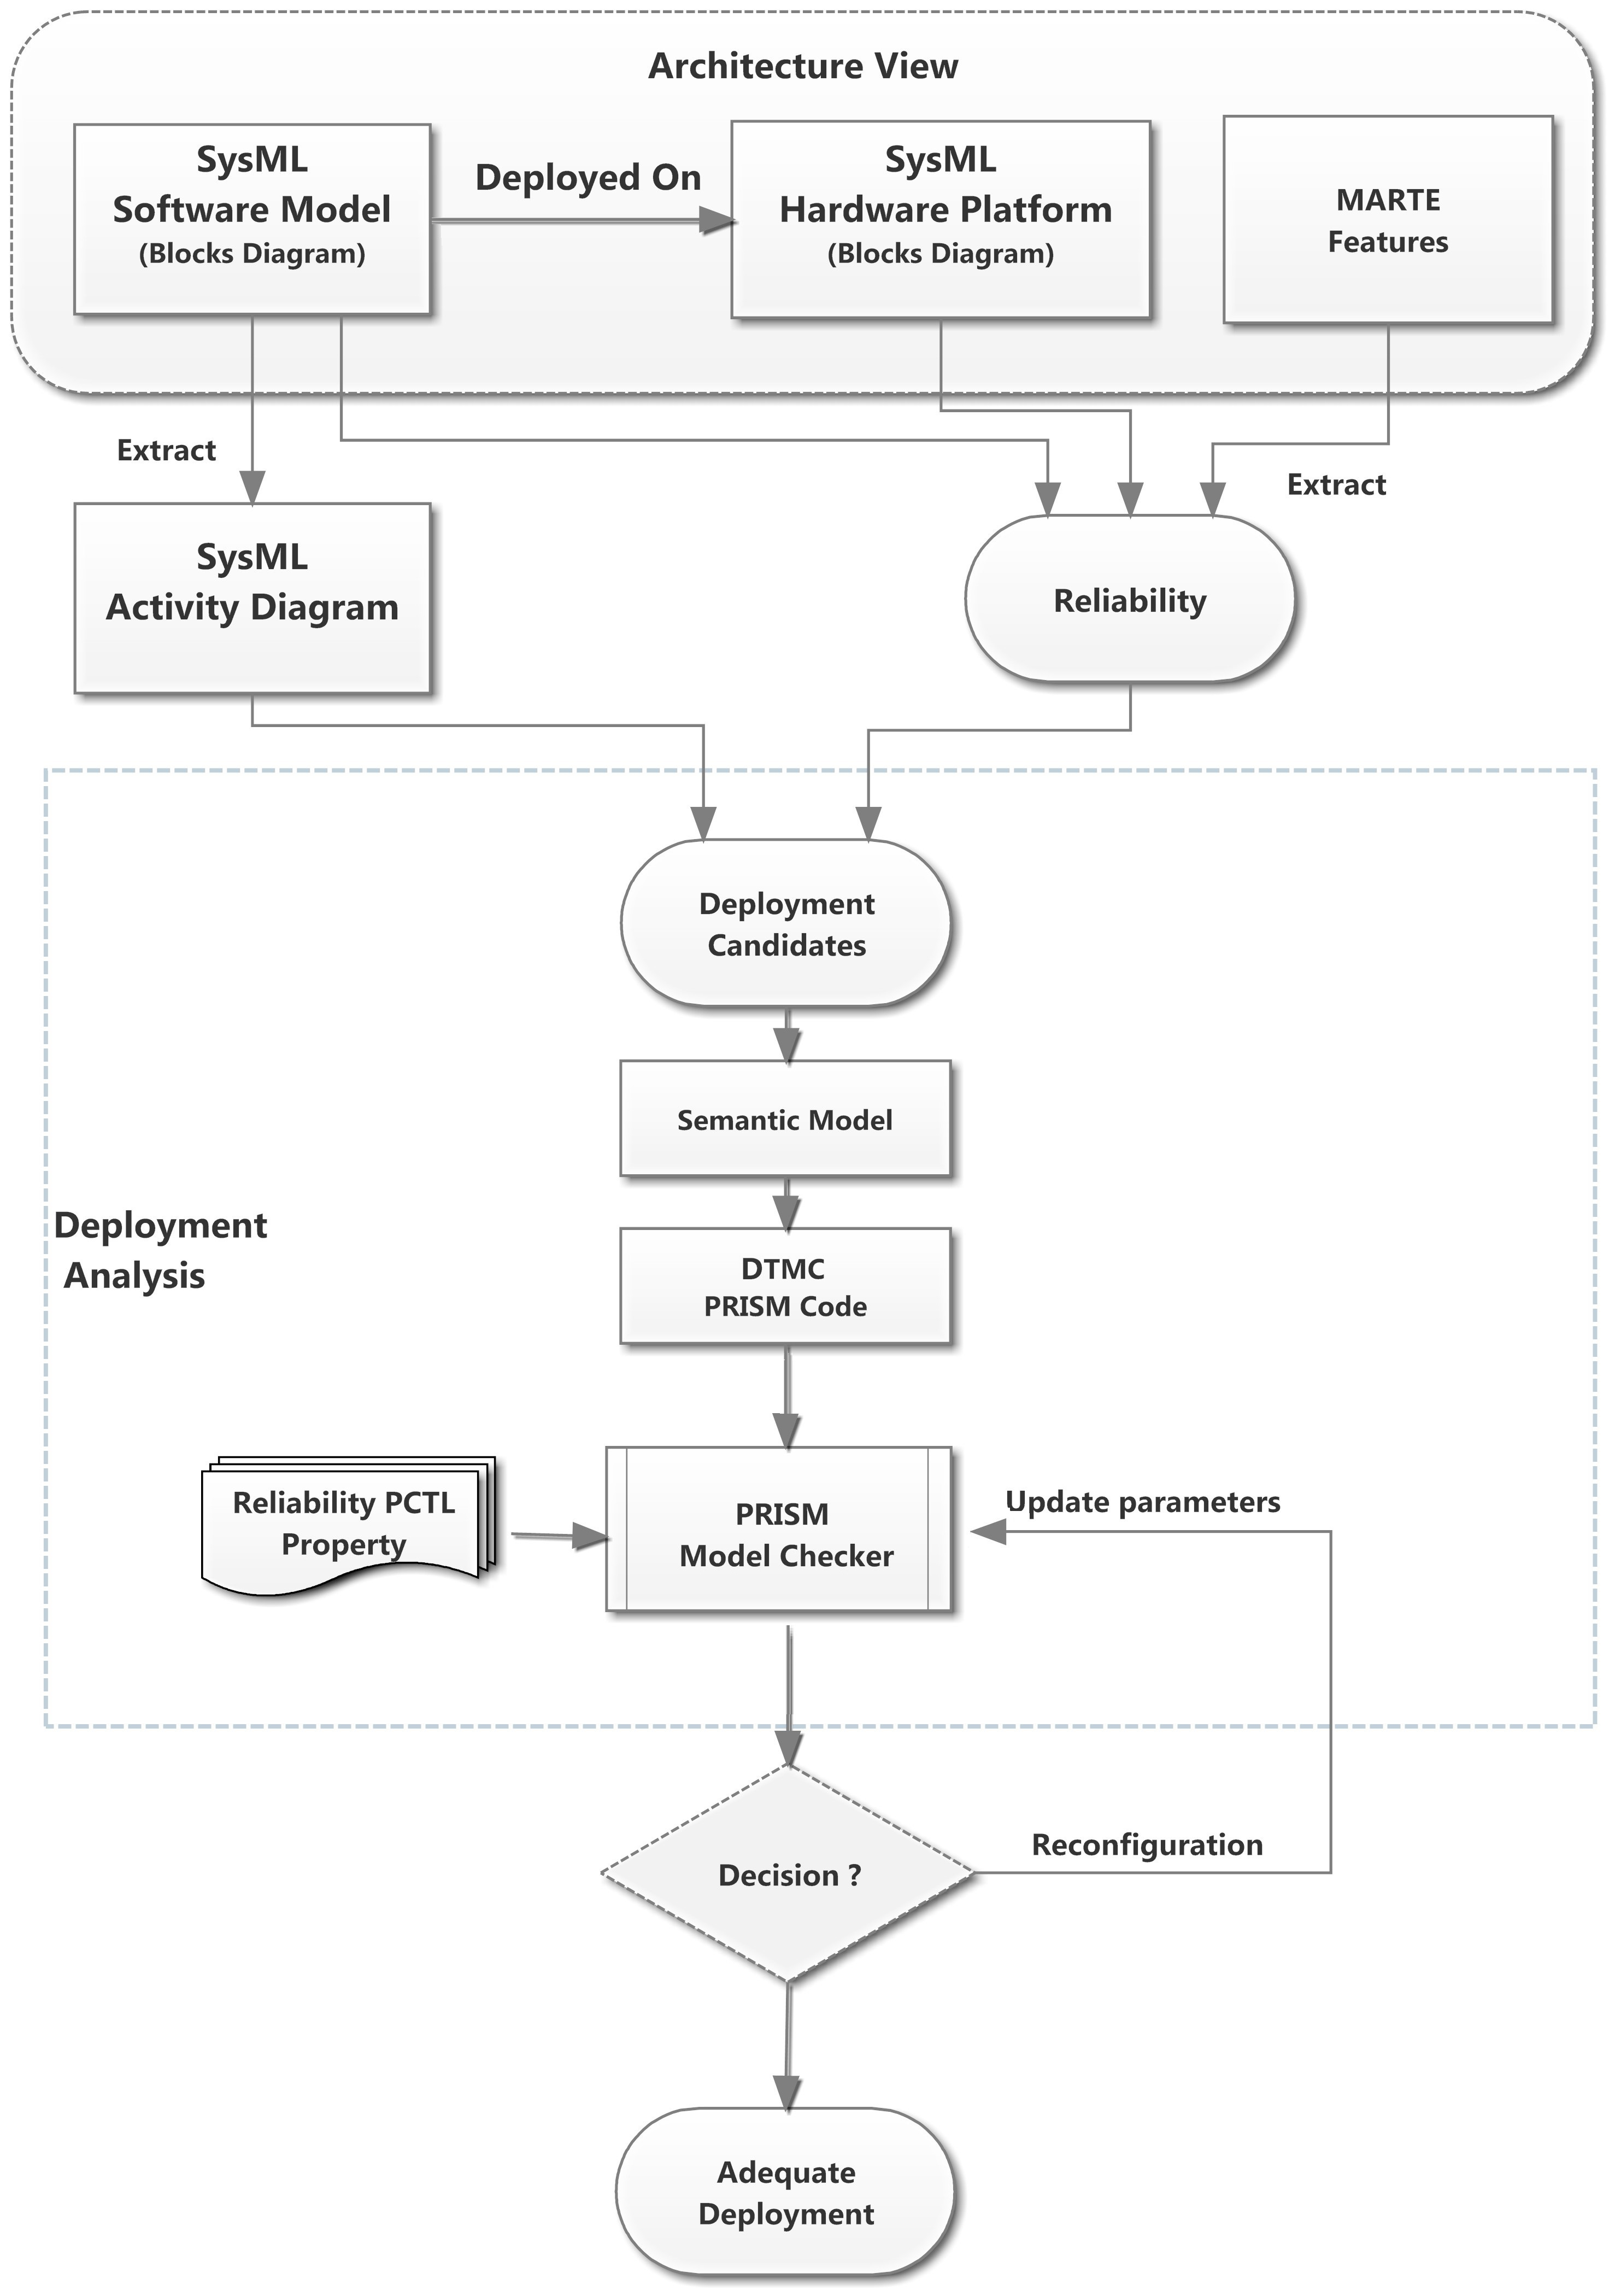
\includegraphics[width=410pt, height =550pt]{Approach.jpg}
	\caption{Reliability-driven Deployment Appoach}	
	\label{approach}
\end{figure}

The remainder of this paper is structured as follows: Section \ref{Automotive Systems} discusses briefly about Automotive Control Systems. Section \ref{DeploymentQualityMeasure} shows how the deployment is resolved according to the designer parameters. Section \ref{Related works} reviews the related work. Section \ref{section3} describes the SysML blocks diagrams and its associated behavior. The PRISM model checker is presented in section \ref{section4}. The internal blocks behavior expressed in activity diagram is formalized in Section \ref{SysMLActivitydiagramformalization}. The
semantics of PRISM models is presented in section \ref{section5}. Section \ref{secverf} provides a mapping algorithm of SysML activity Diagrams into PRISM code and its soundness is proved in section\ref{sound}. Section \ref{section8} illustrates the application of our framework on a case study. In section \ref{section9} our main findings and threats to validity are discussed. Section \ref{section10} draws conclusions and lays out future work.

\section{Automotive control systems}
\label{Automotive Systems}
 The Automotive Control Systems are the \emph{active safety functions} \citep{Reif2014} that encompass all features intended to prevent accidents. The main active functions that are studied in our paper are: Anti-lock Brake (ABS) and Adaptive-Cruise Control (ACC) Subsystems.

\subsection{Adaptive cruise control}
ACC (Adaptive Cruise Control) \citep{Reif2014} simplifies the task of driving a car because it relieves the driver of the mentally demanding task of keeping a check on the car’s speed. The main function of ACC is keeping the speed constant at the setting selected by the driver (i.e. Absence of vehicle in front). In Fig.\ref{ACCbig}, if the vehicle in front is traveling at a constant speed, a car fitted with ACC will follow it at the same speed and a virtually constant distance. That is because the distance between the two vehicles is at least within a broad speed range. Here the speed change is automatic without the need for driver intervention. 

\begin{figure}[!ht]
	\centering
	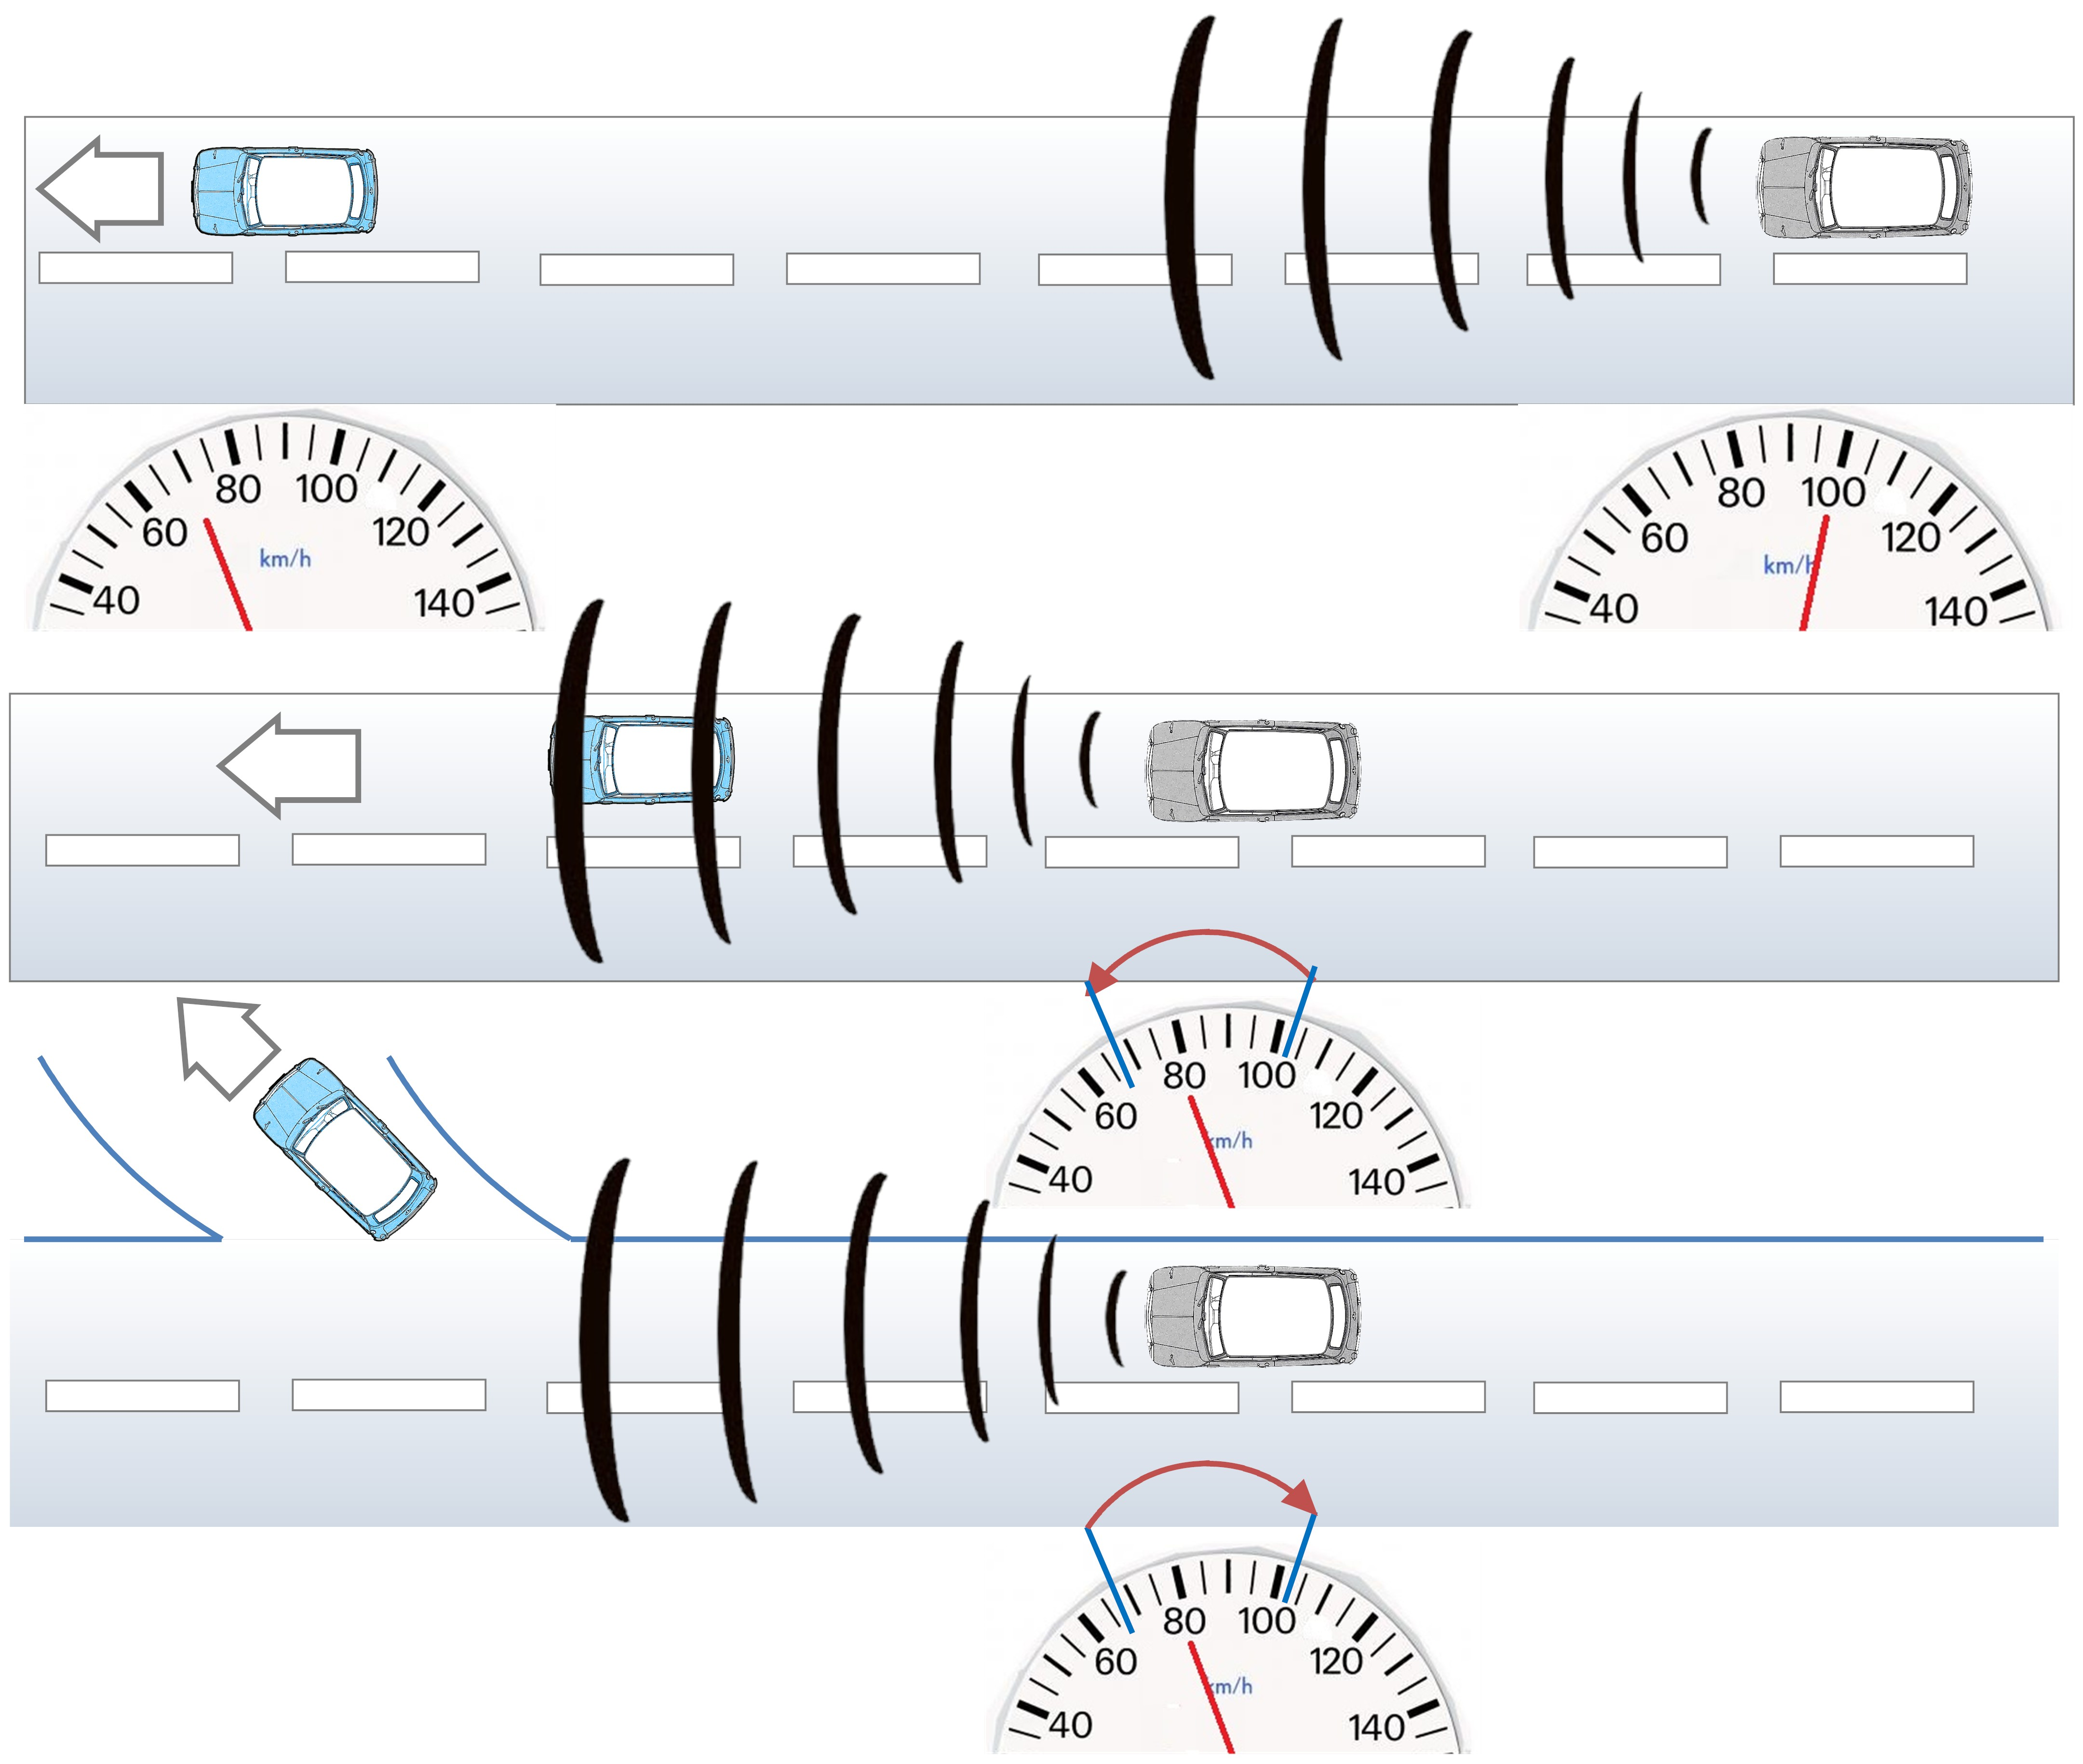
\includegraphics[width=3.2in, height =2.5in]{ACC.jpg}
	\caption{Adaptive Cruise Control System}
	
	\label{ACCbig}
\end{figure}
\subsection{Anti lock brake system}

Wheels of a vehicle may lock up under braking due to wet or slippery road surfaces then the vehicle become uncontrollable and leave the road. The anti-lock braking system (ABS) detects if one or more wheels are about to lock up under braking and if so makes sure that the brake pressure remains constant or is reduced. As a consequence the vehicle can be braked or stopped quickly and safely. The core unit in the system processes the information received from the brake paddle according to defined mathematical procedures. The results of those calculations form the basis for the control signals sent to the emergency stop detection (see Section \ref{section8}).


\section{Solving the deployment problem}
\label{DeploymentQualityMeasure}
According to \citep{Arcangeli2015198}, the deployment is a post-production process that consists in making software available for use and keep it up-to-date and operational. Nevertheless,  current software are organized in as a set of components assembled as a system and operating together \citep{Carlson2006127}. Component-based software must take into account dependencies between components themselves  (i.e. Scheduling and communication) and between software components and its environment (e.g. Execution platform, smartphone). Thus, deployment plan must satisfy a set of constraints to build the correct system. The reference papers on software deployment are those of \citep{Flissi2008} and  \citep{Juve2011}. \citep{Flissi2008} propose \emph{DeployWare} for the deployment of software systems  on nodes of grids. The deployment scheme is described using an architecture description language (ADL) which captures the system configuration. Validation consists of fulfilling all dependencies between software components, avoiding errors and resource conflicts. \citep{Juve2011} target automatic deployment of distributed applications on clouds using \emph{Wrangler}. It allows users to send a simple XML description of the desired deployment consisting of several nodes and services to the cloud coordinator. It manages the provisioning of virtual machines, the installation and the configuration of software and services. The coordinator ensures that the request is valid and all dependencies can be resolved.


In embedded systems, the deployment process consists on automatically explores the states space of possible allocations of software blocks to hardware blocks according to the constraints addressed in this section, and returns the set of near-optimal candidates. In our paper, software deployment is driven by the reliability of the system services that must be maximized. Service refers to the flow of actions and data at software level. We assume that software failures due to programing imperfections are unlikely influence the deployment process, then we may abstract away from the hardware-independent software reliability. In addition, the software and hardware architecture is constant during the deployment.

Our approach assumes that processors are fail silent \citep{Meedeniya2011835}, \citep{HeinerT98}. This means that the processor detects the all errors and switch immediately to passive state which leads to an exception at software level. When failures occur during the execution of a software blocks, it impacts the reliability of our system. With a fixed and deterministic scheduling strategy, any failure happens on processor leads to service execution failure.  

To evaluate a single deployment we use some specification metrics for the software and the platform architecture to capture the system reliability. The constraints established in this section correspond to the attributes of components in SysML specification. For instance, the processor capacity corresponds to the $<<HwProcessor>>$ featured with  MIPS as MARTE annotation (see Section \ref{section3}).


\subsection{Hardware Architecture}
The set of execution components represented by processor are denoted by U =\{ $u_{1}, u_{2},...,u_{m}$ \}, where $m \in \mathbb{N}$ and the parameters of hardware architecture are given as follows:

\begin{itemize}
    \item Processor speed, \emph{ps} : U $ \rightarrow \mathbb{N}$; the instruction-processing capacity of the hardware component in MIPS(million instructions per second). 
    \item Processor failure rate, \emph{$\lambda$} : U $ \rightarrow \mathbb{N}$; the rate parameters of the Poisson distribution that characterizes the probability of a single processor failure. 
    % \item Bus data rate, \emph{dr} : U$ \times $U $ \rightarrow \mathbb{N}$; the data transmission rate of the bus expressed in KBPS (kilobytes per second). 
\end{itemize}

\subsection{Software Architecture}
The set of software components that must be allocated to processor are denoted by C =\{ $c_{1}, c_{2},...,c_{n}$ \}, where $n \in \mathbb{N}$ and the parameters of software components are given as follows:

\begin{itemize}
    % \item Component size, \emph{sz} : C $ \rightarrow \mathbb{N}$; refers to memory size of component used in deployment expressed in KB(kilobytes)  
    \item Component workload, \emph{wl} : C $ \rightarrow \mathbb{N}$; computational requirement for component expressed in MI (millions instructions)
    %\item Data size sent over link, \emph{ds} : C$ \times $C $ \rightarrow \mathbb{N}$; the amount of data transmitted. 
    %\item Initiation probability over link, \emph{q$_{0}$} : C$ \times $C $ \rightarrow  ]0, 1[$	 
    %\item Next-step prob, \emph{p} : C$ \times $C $ \rightarrow ]0, 1[$	 		
\end{itemize}

Let D= \{ d$|$ d:C $\rightarrow$ U \} denotes the set of  all functions assigning software components to hardware processors, and we write a single deployment alternative d$_{j}$ =\{ $(c_{1},u_{j1}), (c_{2},u_{j2}),..., (c_{n},u_{jm})$ \} $\subseteq D$ as  d$_{j}$ =\{ $u_{j1}, u_{j2},..., u_{jm}$ \}.





The quality metric of the approach depends on the reliability of physical hardware (Processors and buses). The reliability of the physical elements in our paper is computed according to failures of execution elements (Processors). The reliability of single element $i$  \citep{Meedeniya2011835} can be modeled with exponential distribution as: 

\begin{equation}
\label{eq1}
\mathrm{R_{i} = e ^{- \lambda . T}}
\end{equation}

where $\lambda$ is the failure rate of the element and T is the time elapsed in it.

In this model, failure rates of execution elements are obtained from the hardware architecture parameters and time taken for the execution is defined as function of the software-component workload and processing speed \citep{Meedeniya2011835}. In time triggered-architecture \citep{HeinerT98}, processing  depends on the fixed scheduling algorithm. Thus, the requests are queued until their time slot is arrived. Based on the software workload and processing speed of the processors, the scheduling length can be calculated as follows:

\begin{equation} sl(u_{i})= \sum_{c\in d^{-1}(u_{i})} \frac{wl(c)}{ps(u_{i})}\end{equation}

The reliability of individual software block are computed as :


\begin{equation}
\label{eq2}
\mathrm{R_{i} =  e} ^{- \lambda(d(c_{i})) sl(d(c_{i}))/2}
\end{equation}


The result $R_{i}$ refers to the reliability of each allocation of software component that allows populating our activity diagram with probabilities or could be a parameters for PRISM model checker. We note that the probabilities on activity diagram are unset (i.e. variables). When the reliability of individual software blocks are known, the full reliability is computed using PRISM model checker applied over the parameterizable activity diagram and we refer to the full reliability as $R_{d_{j}}$. 

Having the reliability measure $R_{d_{j}}$ for each candidate under deployment $d \in D$, the reliability $\mathrm{R}$ of the best candidate is calculates as :

\begin{equation}
\label{eq3}
\mathrm{R}=  Max \{ R_{d_{0}} , . . . . , R_{d_{m}} \}, \ \ \   m \in \mathbb{N}
\end{equation}



\section{Related work}
\label{Related works}

In this section, we depict the recent works related to the deployment, partitioning and allocation optimization then we compare them with our proposed approach.


\cite{Meedeniya2011835} present an approach for reliability optimization in case of software deployment. The inputs are a set of hardware and software constraints (i.e. physical failures, software workload, deployment restrictions) that are considered as inputs for the reliability function. The approach uses Genetic Algorithms (GA) \citep{Sivanandam2010} to optimize the reliability function. This approach is dedicated to be integrated as framework for AADL language (Architecture Analysis and design Language) \citep{5446809} but the authors did not explain how they integrated it in the top of language as an extended properties since AADL supports it.

\cite{Thiruvady20141937} identify the software-to-hardware assignments that maximize the reliability of the system with respect to constraints. These constraints include memory, physical platform failure and communication between software components. The deployment-space exploration is based on Ant Colony Optimization (ACO) combined with constraint programming (CP). However, a predefined number of solutions are constructed to apply CP which is hard for large space of deployment candidates

\cite{Herrera201455} present the COMPLEX approach for hardware/software partitioning and allocation to specific physical platform (i.e. software and hardware). The approach is based on a customized profile. The profile is a UML/MARTE with additional annotation to specify a design-space allocation. However, the authors focus more on the design specification than on partitioning. Also, the authors do not provide any information about algorithm or strategy applied.

\cite{Nascimento2012} present a framework for software- hardware mapping and code generation based on Model-Driven Engineering (MDE) proposed by the Object Management Group (OMG). The approach starts from UML class and sequence diagrams annotated using MARTE profile and use the network of timed automata (i.e. Behavior) as input to the UPPAAL \citep{Behrmann2004} model checking tool for temporal property satisfaction. For design-space exploration. The mapped model is processed by H-SPEX DSE tool \citep{Oliveira2007}. The core of the tool is based on Ant Colony Optimization. However, the authors do not clarify the optimization strategy that is hidden from the user.   


\cite{Brosse2012} present ENOSYS design flow for the Modeling and Synthesis of Embedded Systems. The approach consists of four consecutive steps respectively named Modeling, Synthesis, Source Code Optimization and Design Space Exploration. The modeling step is based on UML Composite diagrams (i.e. Components representations) with the core behavior using state machine or activity diagrams. The composite diagram is enriched with set of annotations using MARTE profile to express the software, hardware components and allocations. Automatic partitioning of the system into software and hardware components occurs when software code is generated and  executed to obtain performances, area and early power figures. These performance characteristics are checked against the required objectives. The process is executed until the required constraints are met. Then, the hardware objects are synthesized directly to VHDL/Verilog whereas the software aspects are compiled for the multi-core CPU platform (i.e. C/C++) which forms the programmable domain of the system implementation. The disadvantages of the approach is that the process of exploration occurs at code level instead on design level which is time consuming. 


\cite{MartinezAlvarez20136813} propose a multi-objectives optimization tool with the Software Hardening Environment for the fault tolerant embedded systems design. The tool automatically transform an original source code (application) into a selective hardened version of the program and return a set of valuable information about the code and execution time overheads, and the fault coverage provided. The optimization tool apply Genetic Algorithm (GA) to fulfill a set of given criteria of interest taking into account fault tolerance parameters.


\cite{Besnard201554} present a verification and validation framework of embedded software using AADL and its behavioral annex. The specification is based on  AADL language(Architecture Analysis and design Language) \citep{5446809} and Simulink \citep{simulink} for functional behavior. The authors implement a systematic translation of the AADL standard and of Simulink diagrams in the multi-clocked synchronous semantics of the Signal data-flow language \citep{Ma2013} that enables timing analysis, formal verification and simulation. Multiprocessor partitioning occurs when the allocation of threads to processors has been achieved with respect to timing constraints that results from scheduling analysis.



\cite{Nath201430} address a partitioning of JPEG encoder (i.e. applied for obtaining high quality output from continuous-tone images) into software and hardware components. The approach is based on multi-objectives optimization taking into account mainly the execution time, the memory requirement, the power consumption. The process  applied the genetic algorithm on control data flow graph (CDFG). However, the specification is based on control data flow graph (CDFG) of 22 components of JPEG encoder.  





\cite{Posadas20141281} present a methodology based on MDE approach to automatically synthesizing the software code of complex embedded systems specified using UML/MARTE model for components diagrams and C code for functional behavior. The synthesis process enables the exploration of different allocations of software components in real physical platforms including processors and memories. By identifying the memory spaces of the components, their interfaces and allocations, it is possible to generate binary files for different allocations from the same inputs and chose which has a positive impact on the total performance of the system. The approach is not really interesting since the decision is made at synthesis level. 

\cite{Jia2014} propose two-phase approach to optimal mapping of real time application on Multiprocessor System-On-chip (MPSoC) platform while considering multiple design constraints. The first phase is heuristic-based for a rapid pruning of the large design space based on partitioning, scheduling and assignment. The reduced number of potential solutions are simulated. Three objectives are optimized: Maximize efficiency in the utilization of processing elements, Minimize the load unbalancing in processing elements and Minimize the communication traffic. The input of the optimization is a set of  software and hardware parameters such as real time constraints and communication delays except the failures of the processing units that are not considered.

\cite{Qadri2016} have applied Fuzzy logic to derive a  multicore architecture based on workload requirements and an optimum balance between throughput and energy of the System-on-Chips. In order  to achieve this, a control parameters are modified dynamically in a reconfigurable SoC, i.e.  Number of cores, Operating frequency and Cache size. Consequently, this approach requires the availability of an appropriate mathematical model for energy estimation in multicore architectures. 

\subsection{Comparison}
As a summary, in Table.\ref{table1} we compare our framework to the existing works by taking consideration six criteria:  specification language, addressed problem, applied algorithm, formalization, soundness and automation. The Specification criteria shows if the design is based on clear user view (i.e.Languages and Models). The second criteria focus on the decision problem (i.e. deployment and partitioning) that the authors want to solve. The applied algorithm indicates the procedure used to solve the problem. Formalization criteria confirms if the approach presents a semantics and formalizes the studied diagrams. Soundness feature shows if the mapping of the studied approach is proved. Automation criteria checks if the presented approach is automatized. From the comparison, we observe that only few works formalize the specification diagrams, including the model checking as decision tool for deployment case. Our work has for objective to support: component-based specification using SysML/MARTE and formalizing the SysML activity diagram. In addition, we implement the tool that allows the automatic deployment decision. 	
\begin{sidewaystable}
	\begin{center}
		
		\begin{tabular}{ l l m{2cm} l   l l l}
			
			\hline
			Approach &  Specification & Problem &  Algorithm & Formalization & Soundness & Automation \\ 
			\hline
	
		\cite{Herrera201455} & UML/MARTE & Partitioning & & & &\multicolumn{1}{c}{$\surd$} \\
	
		\cite{Thiruvady20141937} &  & Deployment & Ant Colony Optimisation & & &\multicolumn{1}{c}{$\surd$} \\
		
		\cite{Meedeniya2011835} &  & Deployment & Genetic Algorithm & & &\multicolumn{1}{c}{$\surd$} \\
		
		\cite{Nascimento2012}  & UML/MARTE & Deployment & Ant Colony Optimisation & \multicolumn{1}{c}{$\surd$}  & &\multicolumn{1}{c}{$\surd$}\\				
		
		
		\cite{Brosse2012}	& UML/MARTE& Partitioning &  & & &\multicolumn{1}{c}{$\surd$}\\	
		
		
		\cite{MartinezAlvarez20136813}	&  & Requirement Optimization & Genetic Algorithm & & &\\	
		
		\cite{Besnard201554}& AADL/Simulink  & Allocation & Scheduling Algorithm  & & &\multicolumn{1}{c}{$\surd$}\\	
		
		
		\cite{Nath201430}&  & Partitioning & Genetic Algorithm & & &\multicolumn{1}{c}{$\surd$}\\	
					
		\cite{Posadas20141281}& UML/MARTE & Deployment &   & & & \multicolumn{1}{c}{$\surd$}\\
	
    	\cite{Qadri2016}&   & Deployment & Fuzzy Logic   & & & \multicolumn{1}{c}{$\surd$}\\
	\cite{Jia2014}&  & Partitioning &   & & & \multicolumn{1}{c}{$\surd$}\\
    
		Our & SysML/MARTE & Deployment & Model Checking &\multicolumn{1}{c}{$\surd$} & \multicolumn{1}{c}{$\surd$} &\multicolumn{1}{c}{$\surd$} \\
		\hline			
			
		\end{tabular}
		\normalsize
	\end{center}
	\caption{Comparison with the existing approaches for design-space exploration}
	\label{table1}
\end{sidewaystable}













\section{Background on SysML diagrams }
\label{section3}

The system specification described in this paper is characterized by following a component-oriented approach \citep{Szyperski2002} for the deployment of software components. In component-based approach, the system is built by the composition of multiples blocks (i.e. component) interacting with each others through a well defined interfaces. In addition, the specification of behavior is based on activity diagrams.

 
\subsection{SysML internal blocks  diagram }
The \textbf{block} \citep{Friedenthal} is the fundamental modular unit for describing system structure in SysML. Internal block diagram (IBD) conveys how the parts of a primitive block must be assembled to create a valid instance of the main block \citep{Delligatti2013}.  The graphical notation of SysML helps designers for the specification of embedded systems using IBD in easy way \citep{Nejati2012}. However, the description needs a more information about the software and hardware blocks to apply analysis such as the processor speed. To provide capabilities that are missing in SysML, MARTE profile is used to specify the required platform resources and their quality of service characteristics.

In the case of our approach, the processor is the main component in the hardware board stereotyped using MARTE ``HW_Processor'' from sub profile Hardware Resource Modeling (HRM) (See Fig.\ref{hardplatform}) and some attributes can be added like \emph{mips} that characterize the instruction-processing capacity. To annotate each processor and bus components with probability of success and failure of  data transmission, we use ``GaStep'' annotation from Generic Quantitative Analysis Modeling package (GQAM) with attribute \emph{prob}. Fig.\ref{hardplatform} represents a multi-processing platform used in our case study where blocks are stereotyped with MARTE annotations.  In our paper, \emph{prob} represents the success of processing and the correct service execution. In Table.\ref{table1Marte}, we show the features studied in the previous section with its corresponding MARTE annotations. In addition, When the blocks are defined, they are endowed with behavior. There are three main behavioral formalisms in SysML: activities, state machines and interactions diagrams. 

%\begin{figure}[!ht]
	%\vspace{2.5cm}
	%\centering
	%\includegraphics[width=150pt]{interface.jpg}
	%\caption{Example of interface }
	%\label{interface}
%\end{figure}


\begin{table}[!ht]
    \begin{center}
        
        \begin{tabular}{ l l }
            
            \hline
            Deployment features  &  MARTE annotations  \\ 
            \hline
            Processor speed &      \emph{mips}\\	
            Processor failure &      \emph{Prob}\\	
            Component workload & \emph{hostDemandOps}\\		
            
            
            \hline			
            
        \end{tabular}
        \normalsize
    \end{center}
    \caption{Software/Hardware Deployment features with their corresponding MARTE annotations}
    \label{table1Marte}
\end{table}



\begin{figure}[!ht]
    %\vspace{2.5cm}
    \centering
    \includegraphics[width=380pt, height =270pt]{platform.jpg}
    \caption{Example of Hardware platform}
    \label{hardplatform}
\end{figure}
\subsection{SysML activity diagram}

SysML Activity diagram \citep{OMG} is a graph-based diagram where activity nodes are connected by activity edges. Fig \ref{fig2} shows the set of interesting artifacts used for verification in our framework. The artifacts consist of activity nodes, activity edges, activity control and  activity partitions. Activity nodes have three type: Activity invocation, objects and control nodes. Activity invocation includes action, call behavior, send/receive signals (objects). The Activity control includes:  initial node, flow final, activity final, fork, merge and join node. Activity edge includes: control flow and object flow. Object flow connects the output pin of one action to the input pin of next action to enable the passage of data. Control flow provides additional constraints on when and in which order the action within an activity will be executed. A token on an incoming control flow enables the execution of an action and offers a control token on outgoing control flow when action completes its execution. Control nodes such as join, fork, merge, decision, initial and final are used to control the routing of control token over edges and specify the sequence of actions (concurrency, synchronization). A set of activity diagram artifacts can be grouped into an activity partition (also known as a \emph{swimlane}). A typical case is when an activity partition represents a block or a part and indicates that any behaviors invoked in that partition are the responsibility of the block or the part. In our paper, we link each sub set of actions to each block of the IBD. Fig.\ref{mpeg} presents an example of the electric motor inverter \citep{Cherfi201442} where different activity artifacts are allocated to blocks. The flows crossing the partitions are a kind of data and events transmission and they are annotated with probabilities. An exception could be generated and handled by the \emph{interruptible region} in the first block.
\begin{figure}[!ht]
	%\vspace{2.5cm}
	\centering
	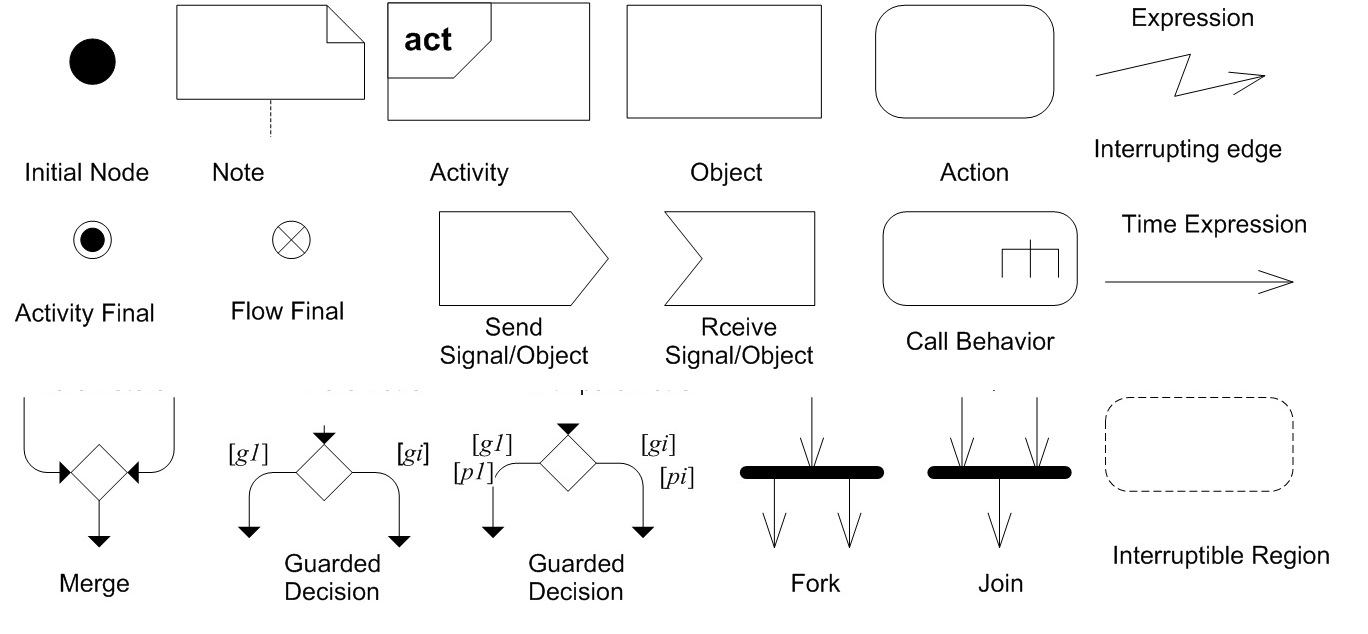
\includegraphics[width=250pt]{artefacts.jpg}
	\caption{A sub set of SysML activity diagram artifacts}
	\label{fig2}
\end{figure}


\begin{figure}[!ht]
	%\vspace{2.5cm}
	\centering
	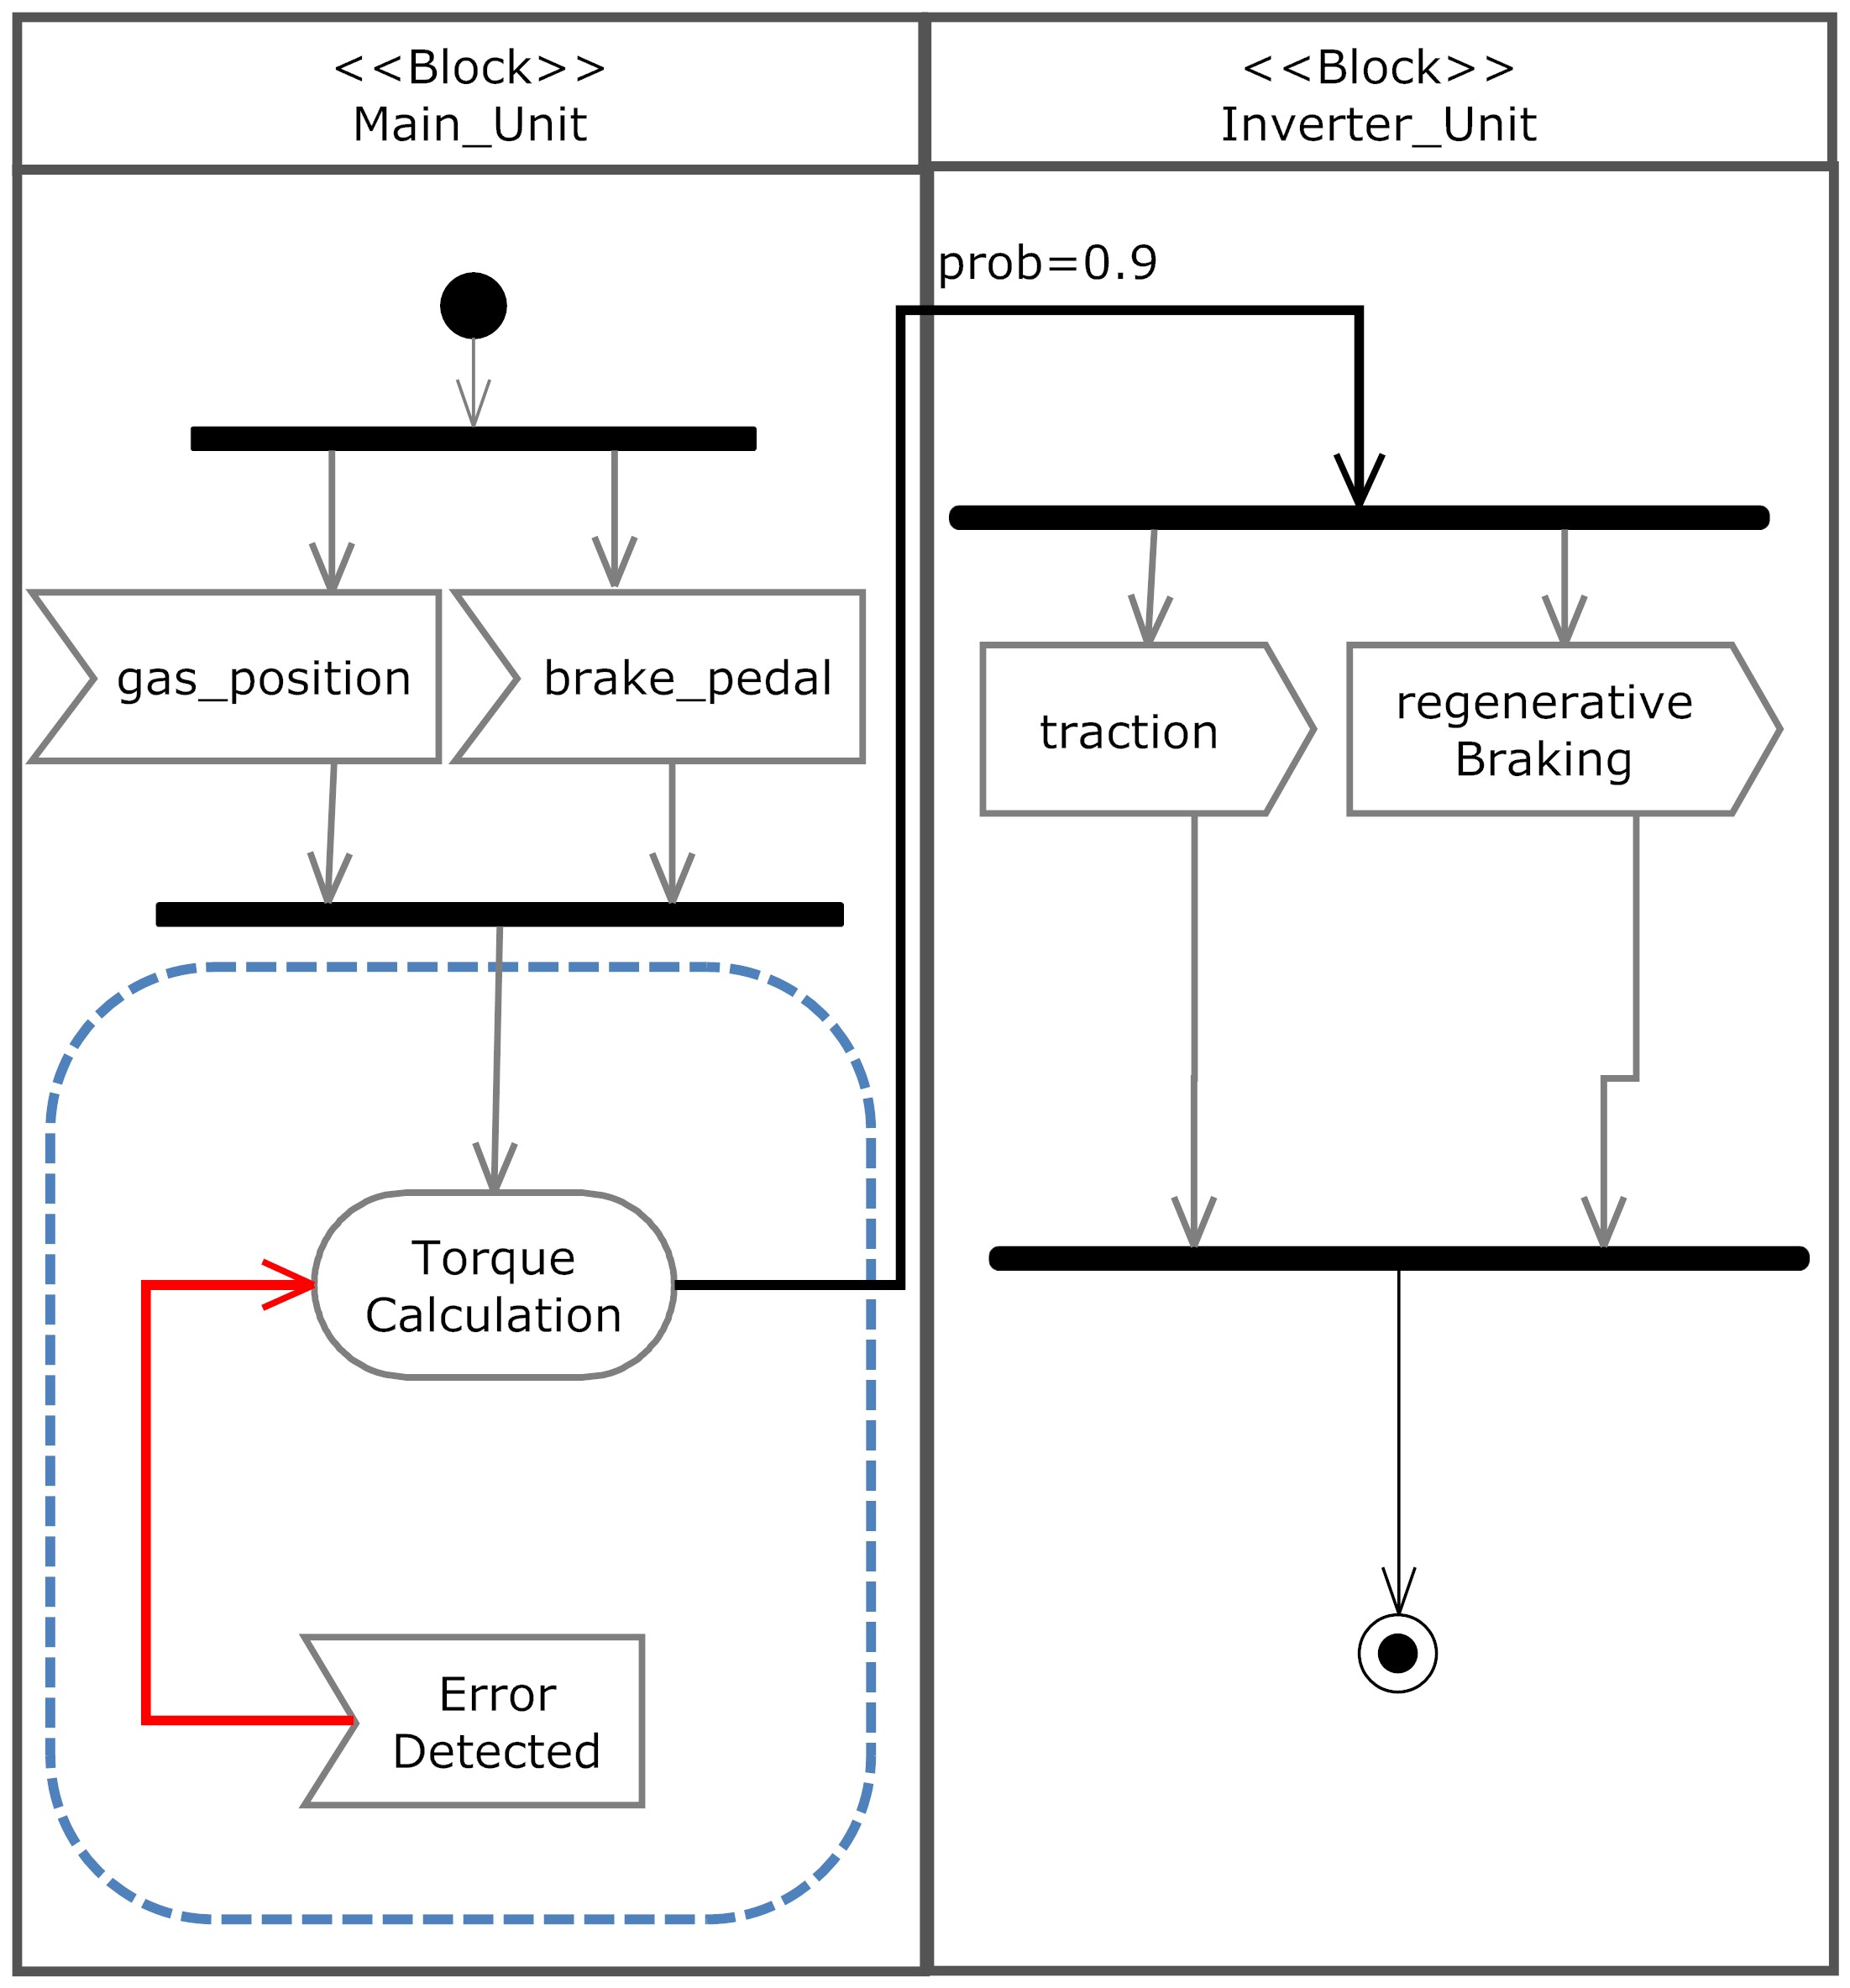
\includegraphics[width=250pt, height =250pt]{vmui.jpg}
	\caption{An example of activity allocated to the blocks}
	\label{mpeg}
\end{figure}






\section{Probabilistic model checking}
\label{section4}

Probabilistic model checking is based on the construction and the analysis of a probabilistic model of system, typically a Markov chain. In this paper, we focus on Discrete-Time Markov chains (DTMCs) with proved usefulness in reliability and availability analysis \citep{Franco2016} \citep{Kwiatkowska2009re}. A DTMC involves as set of states S and a transition probability matrix \textbf{P}: $ S \times S \rightarrow [0, 1] $. The formal definition is:
\theoremstyle{definition}
\newtheorem{mydef}{Definition}
\begin{mydef}Discrete-Time Markov chains (DTMC). DTMC is a tuple M = \textless $\overline{s} $, S, P, L $ >$, where:
\begin{itemize}
	\item $\overline{s} $ \ is an initial state, such that $ \overline{s} \in $ S ,
	\item S is a finite set of states,
	\item P: S $\times  S \rightarrow[0, 1] $ is a rate function assigning for each transition from state $s\ to\ s',\ $ a positive real value $P(s, s') \in [0, 1] $ where $\sum_{s'\in S} P(s, s')= 1$ for all $s' \in S$.
	\item L : S $\rightarrow 2^{AP}$ is a labeling function which assigns to each state $s  \in S$ the set L(s) of atomic propositions that are valid in s.
\end{itemize}

\end{mydef}

Lets consider the case of a Vehicle Management Unit (VMU) \citep{Cherfi201442}. In an electric vehicle, a VMU is responsible for commanding the electric motor inverter, among other functions. With a given certain inputs (gas and brake pedal positions), the VMU sends a torque set point to the inverter that in turn commands the electric motor (traction and regenerative braking), as illustrated in Fig.\ref{mpeg}. In order to prevent an unexpected errors, a watchdog (i.e. a software module) is added which is in charge of bringing the system to a last safe state when errors are detected. The Markov model of such a system as shown in Fig.\ref{auto1example}, is built with two kind of states ($S$: Operational, $S_{f}$: Fault detected) representing the block status. $P$ and $1-P$ are the reliability of correct and failure signal transmission, respectively. This system is described using PRISM modeling language as shown in Listing.\ref{Illustrationsourcecode}.

  	\lstset{
         basicstyle=\ttfamily\footnotesize ,
          caption=Satellite PRISM code,
          frame=single,
          captionpos=b,
          label=Illustrationsourcecode,
          tabsize=2,
          	morekeywords={module,init, endmodule}
        }

        \footnotesize 
        
        \begin{table}[!ht]
         	\begin{center}
            
            
 \begin{tabular}{ p{8cm} }
 \begin{lstlisting}
 const double P;
module satellite
 sc1 :bool init true; // initial node
 .................;
 sf : bool init false;  // final node      
[] sc1 -> (Sfj1'=true)&(sc1'=false);
 .................
[] sf    -> (sc1'=true);
[] sc2 -> (sc3'=true) & (sc2'=false);

[] S -> P:(Ssuccess'=true)&(S'=false)
                +1-P:(Sf'=true)&(S'=false);
               
[] Sf ->(S'=true)&(Sf'=false) ;
[] Ssuccess ->(Sfj2'=true)&(Ssuccess'=false) ;   
 .................
endmodule     
 \end{lstlisting} 	
                
                
                \\
                
                
            \end{tabular}
            
            	\end{center}
        \end{table}
        \normalsize
        

\begin{figure}[!htb]
    \centering
    \begin{minipage}{.5\textwidth}
        \centering
        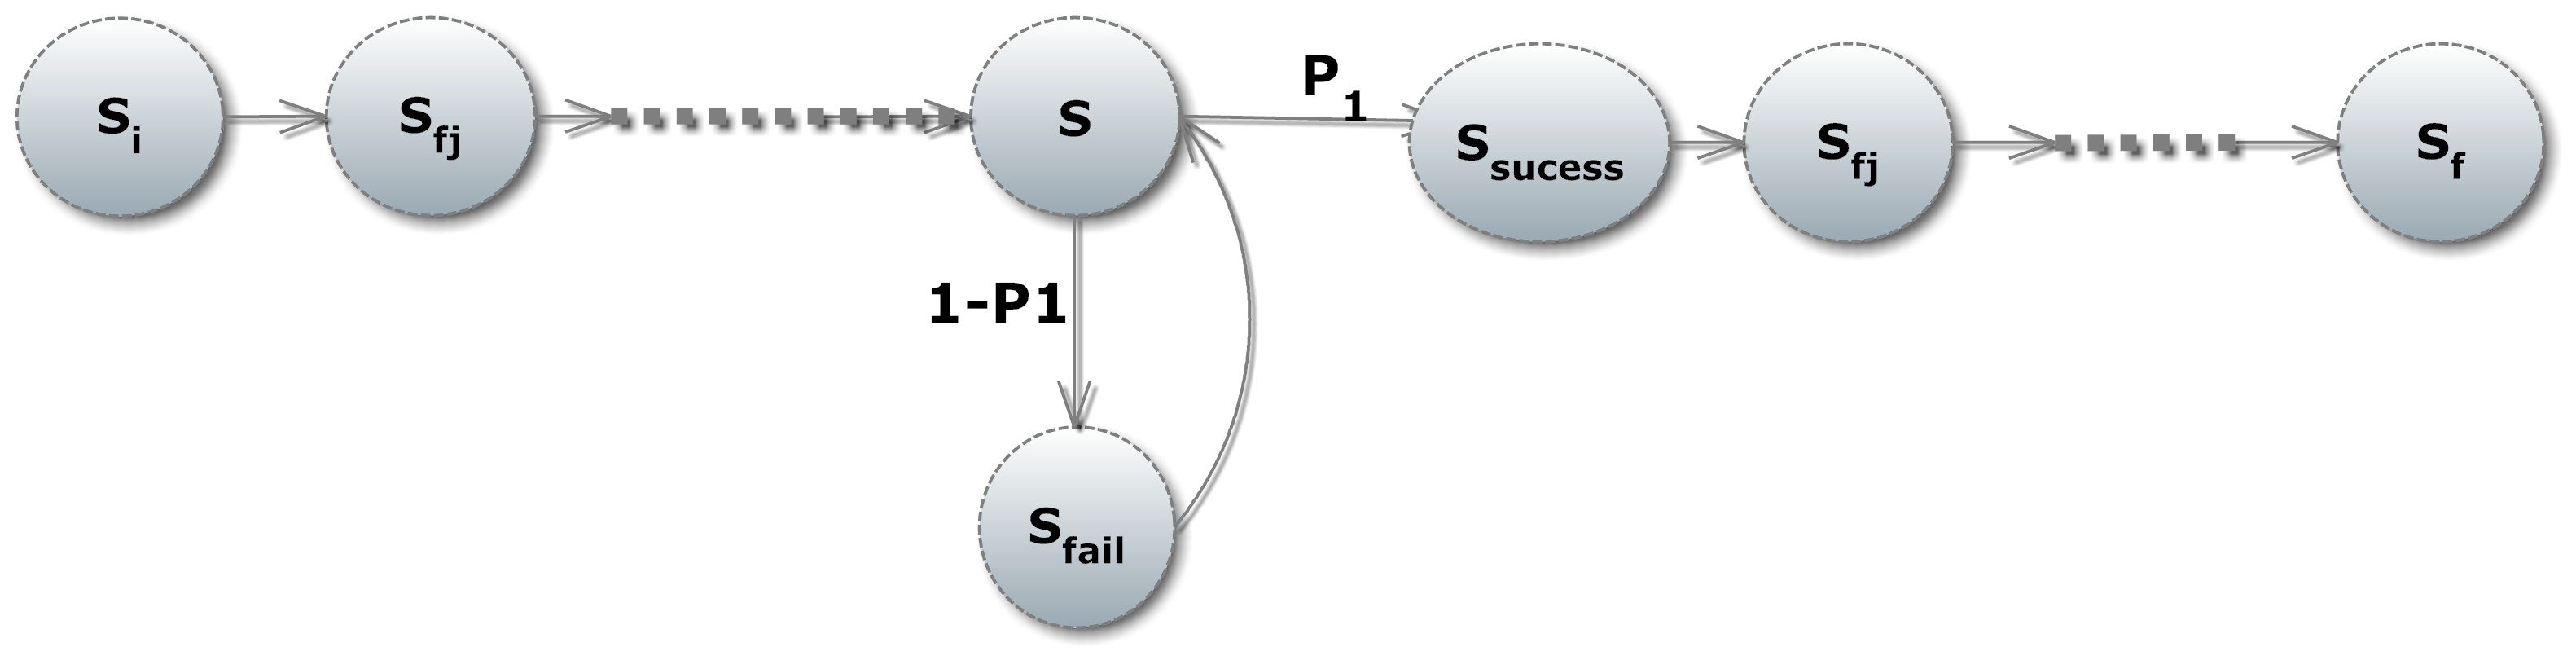
\includegraphics[width=160pt, height =50pt]{dtmcexample.jpg}
        \caption{A simple Markov chain}
        \label{auto1example}
    \end{minipage}%
    \begin{minipage}{0.5\textwidth}
        \centering
        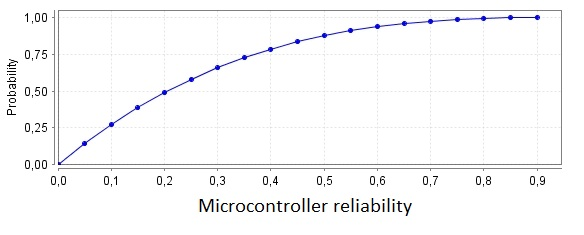
\includegraphics[width=200pt, height =70pt]{reliabilityExp.jpg}
        \caption{Total system reliability}
        \label{auto1examplegraph}
    \end{minipage}
\end{figure}

The model checking approach for reliability analysis requires both a description of system in probabilistic model and properties for performance evaluation using Probabilistic Computation Tree Logic (PCTL) \citep{Kwiatkowska2002}. For the Markov chain in Fig. \ref{auto1example}, if $P$ is parameterizable taking values from 0 to 0.95, then the results could be plotted as graph in Fig.\ref{auto1examplegraph}. The reliability is obtained by checking the model against the property : ``the probability that the system runs correctly within T time steps'' and expressed using PCTL as $P=?[true \cup^{\leq T} S_{success} ], T=100$ ; T is non-negative value representing the upper time bound.  The structure of our temporal logic is expressed by the following BNF grammar:

\subsection{Property Specification}
The syntax of our logic is given by the following grammar:\\

$\varphi$ :: =$ true \ |\ ap \ | \varphi \wedge \varphi \ | \neg  \varphi \  |\  P _{ \bowtie p } [ \psi ]  $,  \\

$\psi$ :: =  $\varphi \cup \varphi \ | \ \varphi \cup ^{\leq k}\varphi  \ , $ \\

Where ``ap'' is an atomic proposition, P is a probabilistic operator. Operator $P _{ \bowtie p } [ \psi ] $  means that the probability of path formula $\psi$ being true always satisfies the bound $\Join $ p, p $\in $ [0, 1]. ``$\Join $''$\in \{ <,\leq,>,\geq \}$. ``$\wedge$ '' represents the conjunction operator and ``$\neg$'' is the negation operator.``$\cup^{\leq k}$'' and ``$\cup$'' are  the bounded until and the until temporal logic operators, respectively.

We use s $\vDash \psi$ to denote that s satisfies the state formula $\varphi$, while $\pi \vDash \psi $ (sequence of states) denotes that $\pi$ satisfies the path formula $\psi$.

\begin{itemize}
	\item $s \vDash$ true is always satisfied,
	\item $s \vDash ap \Longleftrightarrow$  $ap \in L(s)$ and L is a labeling function,
	\item $s \vDash \varphi_{1} \wedge \varphi_{2} \Longleftrightarrow s \vDash \varphi_{1} \wedge s \vDash \varphi_{2}$,
	\item $s \vDash \neg \varphi \Longleftrightarrow s \nvDash \varphi $,
    

	\item $s \vDash P _{ \bowtie p } [ \psi ] \Longleftrightarrow P\{ \pi | \pi\vDash \psi  \}$ such that the probability of the path $\pi =s_{0}...s_{n}$ is given by P($\pi$) = $\prod^{n-1}_{i=0} p(s_{i}, s_{i+1})$,

	\item $s \vDash P _{ \bowtie p } [ \varphi_{1} \cup^{k} \varphi_{2}  ] \Longleftrightarrow \exists i \leq k : \forall j < i, \pi(j)\vDash \varphi_{1} \wedge  \pi(i)\vDash \varphi_{2}$
 
	\item $s \vDash P _{ \bowtie p } [ \varphi_{1} \cup \varphi_{2}  ] \Longleftrightarrow \exists k \geq 0 : \pi \vDash \varphi_{1} \cup^{k} \varphi_{2} $
    \end{itemize}



\section{SysML activity diagram formalization}
\label{SysMLActivitydiagramformalization}
Our methodology enables the search  of the best software-hardware blocks deployment from a parameterizable activity diagram which means; for different deployment candidates, we have different probabilities. The only change occurs on the activity diagram probability values.  To have the best deployment, each candidate with reliability values is checked. Based on \citep{Ouchani20142713} and \citep{Baouya20157493}, we formalize the deployment by developing its calculus : \emph{Deployment Activity Calculus} (DAC). In Table.\ref{rules}, we formally rewrite each SysML activity diagram artifact and each formal notation is identified by a label $\emph{l}$ that belongs to the set of labels denoted by $\mathcal{L}$. We use $\emph{Ex}(p,\mathcal{N}_{1},\mathcal{N}_{2})$ to express an exception that could  happen with probability $1-p$. In this calculus we distinguish between two syntactic concepts: Marked and Unmarked terms. A marked terms are active component with tokens. The unmarked terms correspond to the static structure of the service workflow. We use $\emph{Ex}(p,\mathcal{N}_{1},\mathcal{N}_{2})$ to express an exception that could  happen with probability $1-p$. To describe better our approach, in Table.\ref{rules} we formally rewrite each SysML activity diagram artifact and each formal notation is identified by a label $\emph{l}$ that belongs to the set of labels denoted by $\mathcal{L}$.


For the workflow observations, we use structural operational semantics \citep{Milner1999}  to formally describe how the computation steps of DAC atomic terms take place. We describe the operational semantic rules of the DAC calculus in Table.\ref {op}.  The semantics of parameterizable activity diagram can be described in terms of DTMC as stipulated by Definition \ref{def2}.



\begin{table}[!ht]
	\begin{center}
		\scriptsize
		\begin{tabular}{ m{3cm} m{2.5cm} l}
			
			\hline
			Artifacts & DAC terms & Description \\ 
			\hline
			\raisebox{-0.7cm}{ 
\includegraphics[width=17mm, height=7mm]{elstart.jpg}} 
			
			& $\emph{l} : \emph{i} \rightarrowtail \mathcal{N} $ & Initial node is activated when a diagram is invoked.\\[5ex]
			
			\raisebox{-0.4cm}{ 
\includegraphics[width=4mm, height=4mm]{actfinal.jpg}} 
			
			& $\emph{l} :\odot  $ & Activity final node stops the diagram’ execution.\\[5ex]
			
			\raisebox{-0.4cm}{ 
\includegraphics[width=4mm, height=4mm]{ffinal.jpg}} 
			
			& $\emph{l} :\otimes $ & Flow final node kills its related path’ execution.\\[5ex]
			
			\raisebox{-0.4cm}{ 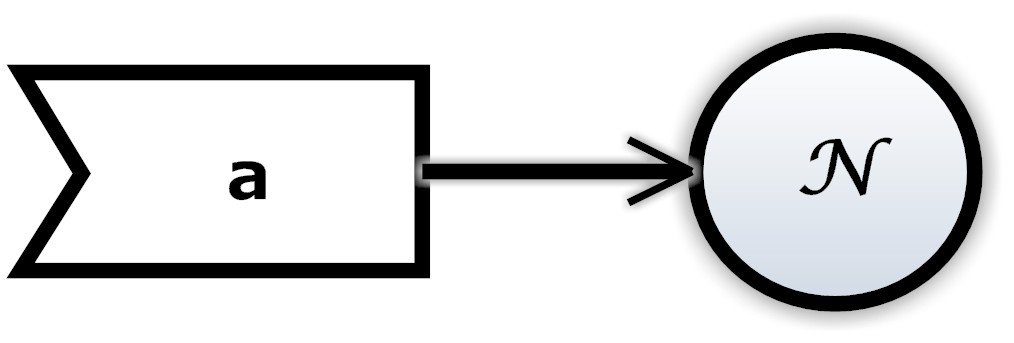
\includegraphics[width=19mm, height=7mm]{receive.jpg}} 
			
			& $\emph{l} : a?v \rightarrowtail \mathcal{N} $ & Receive node is used to receive a signal/object.\\[5ex]
			
			\raisebox{-0.4cm}{ 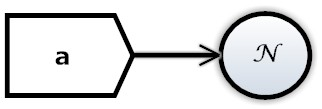
\includegraphics[width=19mm, height=7mm]{send.jpg}} 
			
			& $\emph{l} : a!v \rightarrowtail \mathcal{N} $ & Send node is used to send a signal/object.\\[5ex]
			
			\raisebox{-0.4cm}{ 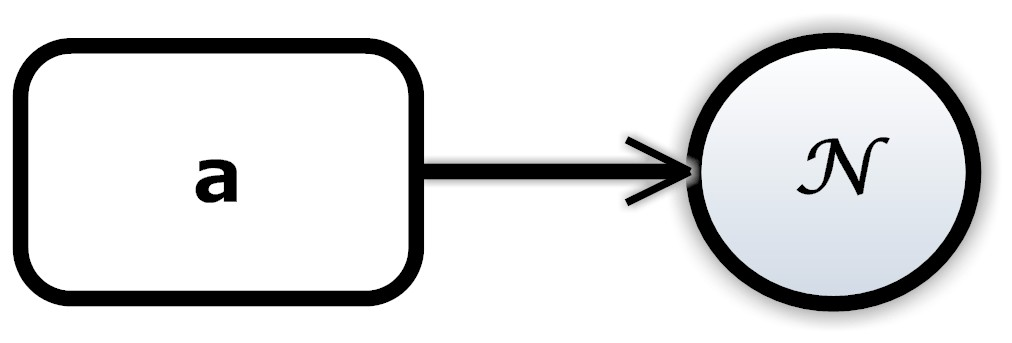
\includegraphics[width=19mm, height=7mm]{action.jpg}} 
			
			& $\emph{l} : a \rightarrowtail \mathcal{N} $ & Action node defines an atomic action.\\[5ex]
			
		
			
			\raisebox{-0.5cm}{ 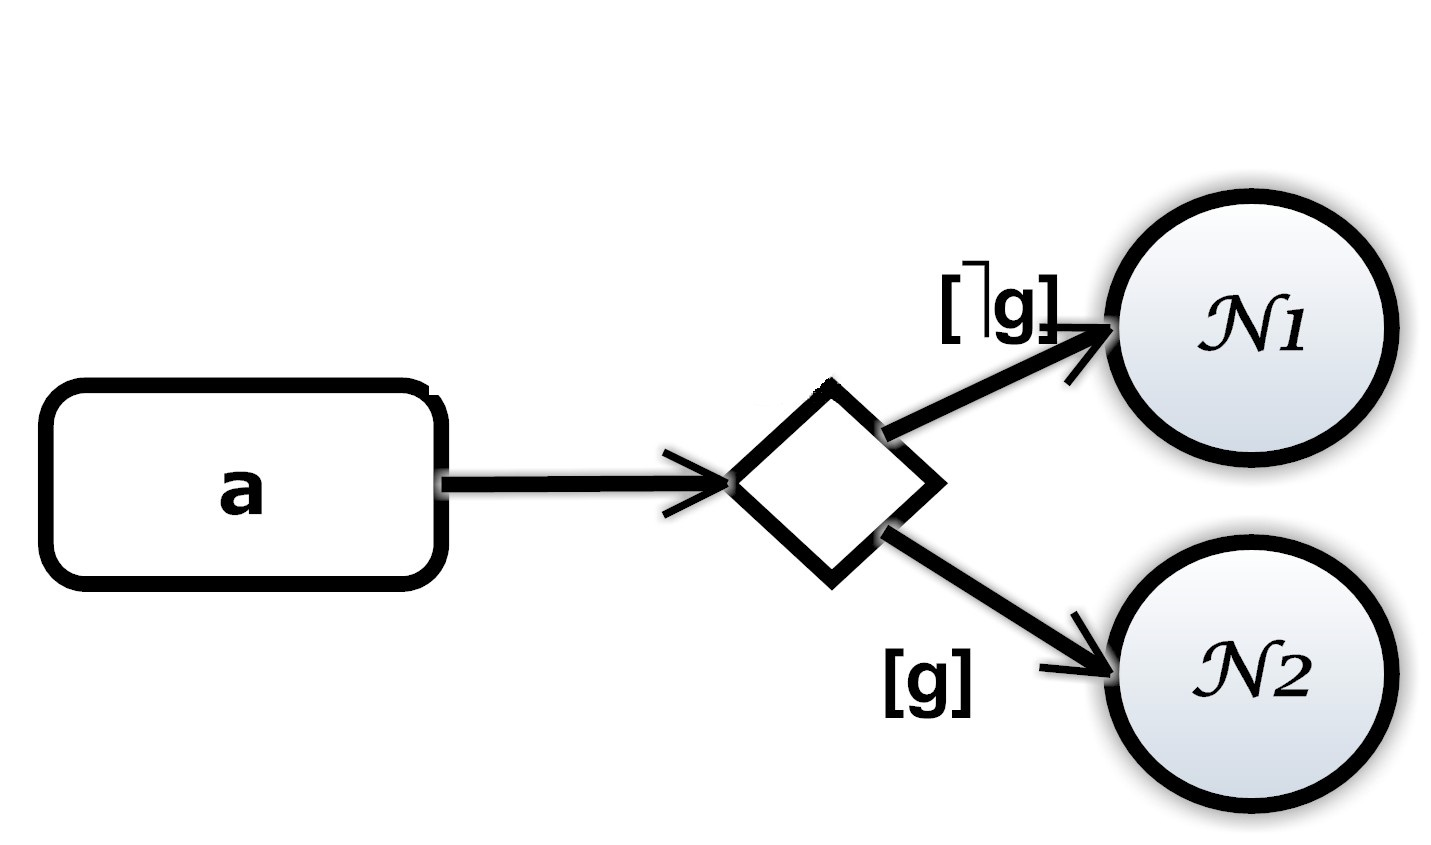
\includegraphics[width=20mm, height=14mm]{decision.jpg}} 
			
			& $\emph{l} : D(g,\mathcal{N}_{1},\mathcal{N}_{2})$ & Decision node with guarded edges $\left\{g,\neg g\right\}$.\\	[5ex]
			
			\raisebox{-0.4cm}{ 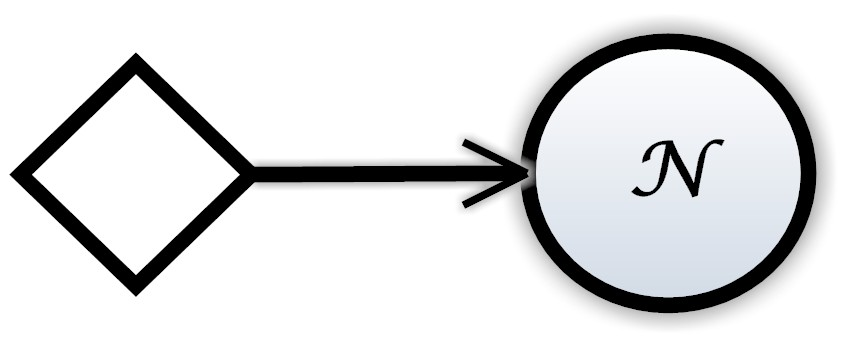
\includegraphics[width=17mm, height=6mm]{merging.jpg}} 
			
			&  $\emph{l} : M(x) \rightarrowtail \mathcal{N} $ & Merge node specifies the continuation and $x = \left\{x_{1}, x_{2} \right\} $ is a set of input flows.\\	[5ex]		
			
			\raisebox{-0.4cm}{ 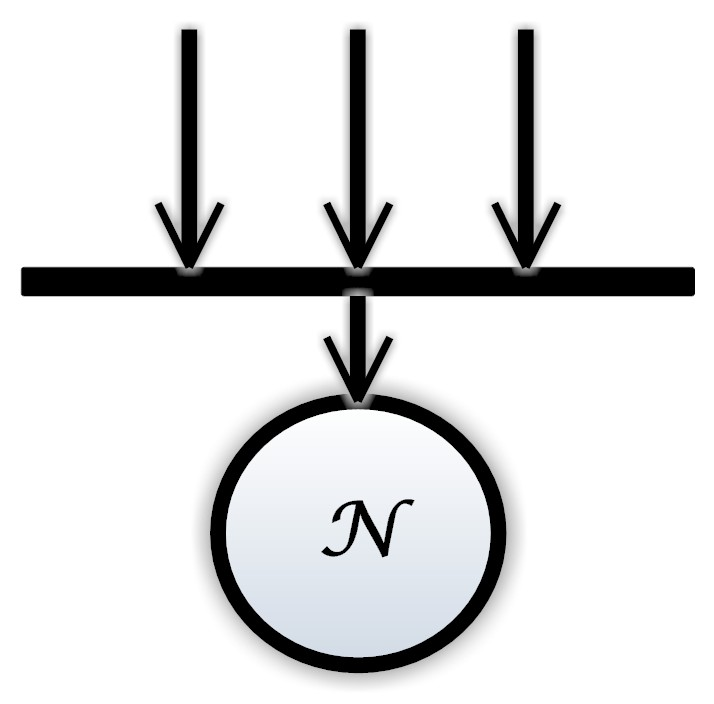
\includegraphics[width=13mm, height=12mm]{eljoin.jpg}} 
			
			&  $\emph{l} : J(x) \rightarrowtail \mathcal{N} $ & Join node presents the synchronization where $x = \left\{x_{1}, x_{2} \right\} $ is a set of input pins.\\	[5ex]
			
			\raisebox{-0.4cm}{ 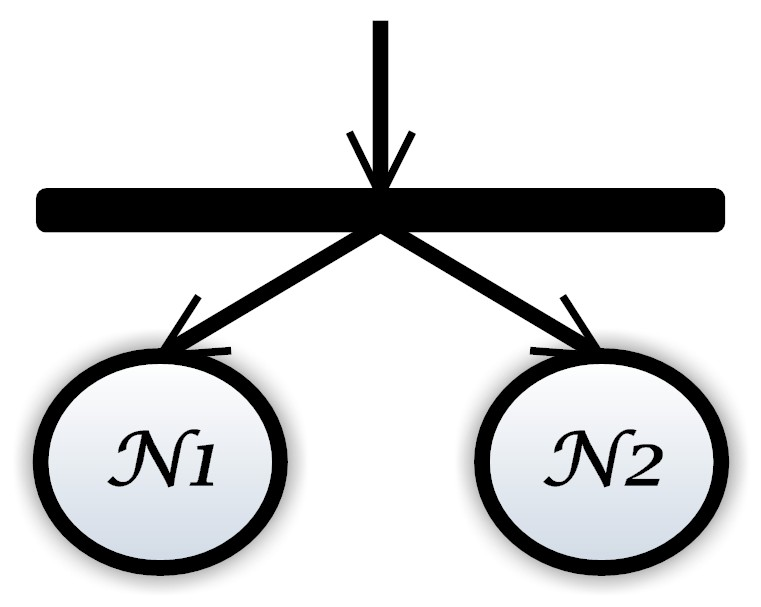
\includegraphics[width=14mm, height=11mm]{elfork.jpg}} 
			
			&  $\emph{l} : F(\mathcal{N}_{1},\mathcal{N}_{2} ) $ & Fork node models the concurrency that begins multiple parallel control threads.\\	[5ex]	
			
            \raisebox{-0.4cm}{ 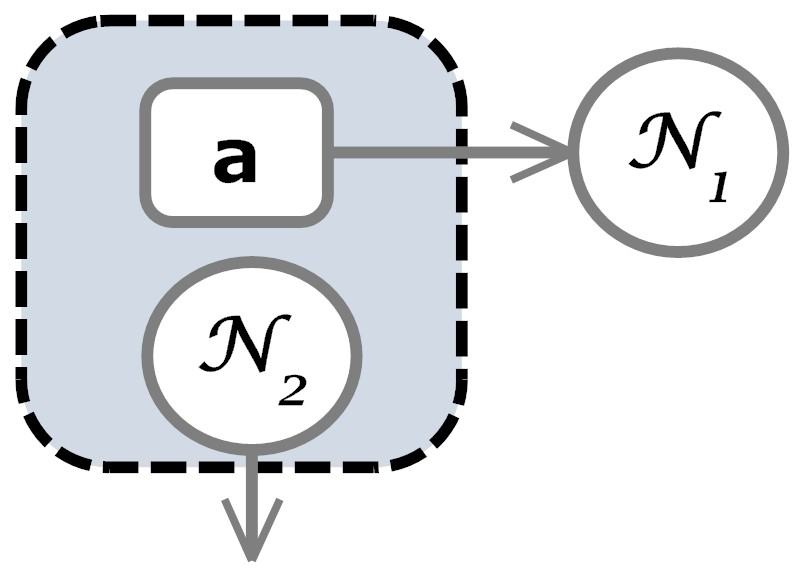
\includegraphics[width=17mm, height=13mm]{interrupt.jpg}} 
                
                &  $\emph{l} : Ex( p_{1},\mathcal{N}_{1},\mathcal{N}_{2} ) $ & Interruptible region models the interruption when errors occurs with $1-p_{1}$\\	[5ex]
			
			
			\hline
			
		\end{tabular}
	\end{center}
	\caption{DAC Terms of SysML Activity Diagram Artifacts.}
	\label{rules}
\end{table}




%%%%
\begin{table}[ht]
	\begin{center}
		\scriptsize
		\begin{tabular}{ m{7cm} m{7cm} }
			
			
			\textbf{INT-1} $\emph{l} : \emph{i} \rightarrowtail \mathcal{N} \stackrel{l }{\rightarrow}_{1} \emph{l} : \overline{i} \rightarrowtail \mathcal{N} $
			This axiom introduces the execution of $\mathcal{A}$ by putting a
			token on \emph{i} .
			&
			\textbf{INT-2} $\emph{l} : \overline{i} \rightarrowtail \mathcal{N} \stackrel{l }{\rightarrow}_{1} \emph{l} : \emph{i}\rightarrowtail \mathcal{\overline{N}} $
			This axiom propagates the token in the marked term \emph{i} into its outgoing $\mathcal{N}$.
			\\
			\textbf{ACT-1} $ \forall n>0, m \geq 0 \ \emph{l} : \overline{\overline{a^{m}} \rightarrowtail \mathcal{N} }^{n} \stackrel{l }{\rightarrow}_{1} \emph{l} : \overline{\overline{a^{m+1}} \rightarrowtail \mathcal{N} }^{n-1}$
			This axiom propagates the token from the global marked term to \emph{a}.

&
			\textbf{ACT-2} $l:  \overline{\overline{a}^{m+1} \rightarrowtail \mathcal{N} }^{n}  \stackrel{l}{\rightarrow}_{1} \emph{l} : \overline{\overline{a}^{m} \rightarrowtail \overline{\mathcal{N}} }^{n}$
			This axiom propagates the token from the marked term a to $\mathcal{N}$.
\\

			\textbf{ACT-4} $ \forall n>0, m \geq 0 \ \emph{l} : \overline{\overline{a}^{m} \rightarrowtail \mathcal{N} }^{n} \stackrel{l }{\rightarrow}_{1} \emph{l} : \overline{\overline{a}^{m+1} \rightarrowtail \mathcal{N} }^{n-1}$
			This axiom propagates the token from the global marked term to \emph{a} with probability p (i.e. failure rate).
&
			\textbf{FRK-1} $  \forall n>0 \ \emph{l} : \overline{F(\mathcal{N}_{1}, \mathcal{N}_{2})}^{n} \stackrel{l }{\rightarrow}_{1} \emph{l} : \overline{F(\overline{\mathcal{N}_{1}}, \overline{\mathcal{N}_{2}})}^{n-1} $
			The FRK-1 axiom shows the multiplicity of the arriving tokens according to the outgoing sub-terms
			\\
			%%%%%%%%%%%%%%%%%%%%%%%%%%%%%%%%%%%%%%%%%%%%%%%%%%%%%%%%%%%%%%%%%%%%%%%%%%%%%%%


			
			\textbf{DEC-1}  $   \forall n>0 \ \emph{l} : \overline{D(g,\mathcal{N}_{1}, \mathcal{N}_{2})}^{n} \stackrel{g}{\rightarrow} \emph{l} : \overline{D(g,\overline{\mathcal{N}_{1}}, \mathcal{N}_{2})}^{n-1} $
			The axiom DEC-1 describes a non-probabilistic decision where a token flows through the edge satisfying its guard.
			
			&
		

			\textbf{EXP-1} $ \emph{l} :  \overline{Ex(\mathcal{N}_{1}, \mathcal{N}_{2} )}^{n} \stackrel{l}{\rightarrow} \emph{l} :  \overline{ Ex(\mathcal{N}_{1}, \overline{\mathcal{N}_{2}} )}^{n-1}$ Node $\mathcal{N}_{2}$ is triggered after an exception
            \\
			
			
			\textbf{EXP-2} $ \emph{l} :  \overline{Ex(p,\mathcal{N}_{1}, \mathcal{N}_{2} )}^{n} \stackrel{l}{\rightarrow}_{1-p}  \emph{l} :  \overline{ Ex(p,\mathcal{N}_{1} \overline{\mathcal{N}_{2}} )}^{n-1}$ Node $\mathcal{N}_{2}$ is triggered after an exception with probability $1-p$.
			
			&
			%%%%%%%%%%%%%%%%%%%%%%%%%%%%%%%%%%%%%%%%%%%%%%%%%%%%%%%%%%%%%%%%%%%%%%%%
			\textbf{MRG-1} $  \emph{l} : \overline{\overline{\mathcal{N}} \rightarrowtail l':M(x,y)}^{n}  \stackrel{l}{\rightarrow} \emph{l} : \overline{\mathcal{N} \rightarrowtail l':M(\overline{x},y)}^{n}$
			MRG-1 is a transition with  rate value equal 1 to put a token coming from the sub-term $\mathcal{N}$ on merge labeled by l.
			\\
			
			\textbf{MRG-2} $  \emph{l} : \overline{M(\overline{x},\overline{y}) \rightarrowtail \mathcal{N}}^{n}  \stackrel{l}{\rightarrow} \emph{l} : \overline{M(x,\overline{y}) \rightarrowtail \overline{\mathcal{N}}}^{n}  $
			MRG-2 is a transition with  rate value equal 1 to present a token flowing from  merge labeled by l to the sub-term $\mathcal{N}$.
			
			&
		

			\textbf{JOIN-1} $  \emph{l} : \overline{\overline{\mathcal{N}} \rightarrowtail l':J(x,y)}^{n}  \stackrel{l}{\rightarrow} \emph{l} : \overline{\mathcal{N} \rightarrowtail l':J(\overline{x},y)}^{n}$ JOIN-1 represents a transition with rate value equal 1 to activate the pin x in a 	join labeled by l
			\\
			
			\textbf{JOIN-2} $  \emph{l} : \overline{J(\overline{x},\overline{y}) \rightarrowtail \mathcal{N}}^{n}  \stackrel{l}{\rightarrow} \emph{l} : \overline{J(x,y) \rightarrowtail \overline{\mathcal{N}}}^{n}  $ JOIN-2 represents a transition with rate value equal 1 to move a token in join to the sub-term $\mathcal{N}$


			&
			\textbf{SND} $  \emph{l} : \overline{a!v}^{n} \rightarrowtail \mathcal{N} \stackrel{l}{\rightarrow} \emph{l} : \overline{a!v}^{n-1} \rightarrowtail \overline{\mathcal{N}} $ SND describes the evolution of the token after sending
			an object $v$.
			
			\\
			%%%%%%%%%%%%%%%%%%%%%%%%%%%%%%%%%%%%%%%%%%%%%%%

		
			\textbf{AFIN}  $ \mathcal{A}[l:\overline{\mathcal{\odot}}] \stackrel{l}{\rightarrow} |\mathcal{A}|$
			This axiom states that if the sub-term $l : \odot$  is reached then no action is taken later by destroying all tokens.
			&

			\\	
		\end{tabular}
	\end{center}
	\caption{Operational semantic rules of the DAC calculus}
	\label{op}
\end{table}













\begin{mydef}[DAC-DTMC]\label{def2} A discrete-time  Markov Chain of DAC term $\mathscr{A}$ is the tuple $M_{\mathscr{A}} = \textless \overline{s} , \textsl{S}, \textsl{P}, \textsl{L}  >$, where:

\begin{itemize}
	\item $\overline{s} $ \ is an initial state, such that $ L(\overline{s}) = \left\{l: \overline{i} \rightarrowtail \mathcal{N} \right\}$ ,
	\item S is a finite set of states reachable from $\overline{s} $, such that, $S =\left\{s_{i:0\leq i\leq n}| L(s_{i})=\left\{ \overline{\mathcal{N}}\right\} \right\} $,

\item	P: S $  \times$ S$'\rightarrow [ 0, 1] $ is a probability function assigning for each  transition from $ s$ to $s' $  a  positive real value $ p$ where:  For each S' $\subseteq$ S such that S'=$\left\{s_{i}:0\leq i \leq n:s\rightarrow_{p_{i}} s_{i} \right\}$ , each transition $s\rightarrow_{p_{i}} s_{i}$  satisfies one DAC semantic rule and  $\sum^{n}_{i=0} p_{i}= 1$.

	
	\item L : S $\rightarrow 2^{[[\mathcal{L}]]}$ is a labeling function where: $[[\mathcal{L}]] : \mathcal{L} \rightarrow \left\{true, false\right\}$.
\end{itemize}

\end{mydef}
  

\section{The PRISM model checker}
\label{section5}
In this paper, we use PRISM probabilistic model checker \citep{Kwiatkowska}. It supports the analysis type of probabilistic models: Discrete-time Markov chains (DTMC) \citep{KP12}, Continuous-time Markov chains (CTMC) \citep{KNP07a}, Markov decision process (MDP) \citep{Forejt2011}.  Since Discrete-timed Markov chains (DTMCs) is considered as appropriate semantic model for modeling reliability \citep{Franco2016} in SysML Activity Diagram, we briefly review the concepts of DTMC. 

A PRISM program ($\mathscr{P}$) is a composition of one or more modules. The state of each module is defined by a set of fined ranged variables $V$. The global state of the system is determined by evaluating the values of those module variables. The behavior of each module is described using commands which include a \textbf{guard} and one or more updates of the form: $$[ ]\mathrm{guard} \rightarrow p_{1} :u_{1}..+ p_{n}:u_{n}$$  The \textbf{guard} is a predicate over the variables of all the modules in the model and \textbf{\emph{$p$}}  is a probability value. Each  update \textbf{\emph{u}} describes a transition which the module can make if the guard is true as assignments form $(V'_{1}=val_{1})$\&..\&$(V'_{k}=val_{k}) $ where $ V_{i} \in \left[min. . .max\right] $  such that $min, max \in \mathbb{N}$ and min $<$ max,  and $val_{j} $ are values evaluated via expressions denoted by "eval" eval: V $ \rightarrow \mathbb{N} \cup \left\{True, False\right\}$.

Definition \ref{pdtmc} stipulates the formal definition of PRISM probabilistic timed automata denoted by $\mathrm{M}_{\mathscr{P}}$. The states of $\mathrm{M}_{\mathscr{P}}$ take the form $\left\langle V_{1}, . . . , V_{k}, eval\right\rangle$. The stepwise behavior of $\mathrm{M}_{\mathscr{P}}$ is described by the operational semantic rules provided in \citep{Baouya20157493}.

\begin{mydef}[PRISM-DTMC] \label{pdtmc} A Discrete-Time Markov Chain (DTMC) of PRISM program $\mathscr{P}$ is the tuple $\mathrm{M_{\mathscr{P}}=< s_{i} , \textsl{S}, P , L >}$, where:

\begin{itemize}
	\item $s_{i} $ \ is an initial state,
	\item S is a finite set of states reachable from $s_{i} $, such that, $S =\left\{s_{i:0\leq i\leq n}| L(s_{i}) \in \left\{ AP\right\}\right\}$,
    
	\item	P: S $  \times$ S$\rightarrow [0,1] $ is a probabilistic function where $\sum_{s'\in S}\mathrm{P(s,s')}=1$ for all  $s\in$ S,
	
	
	\item L : S $\rightarrow 2^{AP}$ is a labeling function that assigns for each state a set of valuated propositions.
\end{itemize}
 \end{mydef} 
\section{Translation rules}
\label{secverf}



This section describes the transformation of SysML Activity diagrams $\mathscr{A}$ into a DTMC written in PRISM input language. We apply an  Algorithm  that takes $\mathscr{A}$ as input and returns its PRISM code. For further details about this algorithm, consult \citep{Ouchani20142713}.   The diagram $\mathscr{A}$ is visited using a depth-first search procedure (DFS) without backing to the visited node and the algorithm's output produces PRISM modules. 

The function $\Gamma$ presented in Listing.\ref{prismcommands} produces the appropriate PRISM commands for each DAC term. The action label of a command is the label of its related term ``n''. The guard of this command depends on how the term is activated. The flag related to the term is its label $l$ that is initialized to false except for the initial node it is true which conforms to the premise of the DAC rule ``INIT-1''. The updates of the command deactivate the propositions of the term, activate that ones related to its successors. For a term $n \in \mathscr{A}$, we define a useful function: $L(n)$ that returns the label of a term n. 

For example, the exception ``$l : Ex(p, N_{1}, N_{2}) $'' (line 29) produces two commands (line 31-32). The first one in (line 31) produces a PRISM command that refers to the correct state transition. Similarly, the second command in (line 32) refers to an exception that may occur with probability $1-p$. This command represents the DAC rule ``EXP-1''.  The DAC term ``$l : D(g, N_{1}, N_{2}) $'' produce two commands in (line-26). The first command is executed when the guard is verified else the second one is executed which follows the DAC rule ``DEC-1''. The generated PRISM fragment of each diagram $\mathscr{A}$ is bounded by two PRISM primitives: the module head ``module $\mathscr{A}$'', and the module termination ``endmodule''.


\lstdefinestyle{customc}{
    basicstyle=\sffamily\small,
    numbers=left,
    numberstyle=\small,
    numbersep=3pt,
    mathescape,
    frame=single,
    caption=Generating PRISM Commands Function,
    captionpos=b,
    linewidth=14cm,
    columns=fullflexible,
    xleftmargin=1cm,
    framexleftmargin=0.5cm
}


\lstset{style=customc,
    label=prismcommands
}

\begin{table}
    \begin{center}
        
        \begin{tabular}{ p{15cm} }

			\begin{lstlisting}
$\mathbf{\Gamma: \mathscr{A}\longrightarrow  \mathscr{P}}$ 
$\Gamma(\mathscr{A})= \forall n \in \mathscr{A}$ , $L(n=\emph(i))= true$, $L( n \neq\emph(i) )= false$
			
 $\textcolor{red}{l : i \rightarrowtail \mathcal{N} } \Longrightarrow $
 $\textbf{in}$
			$ \left\{ [l] l \longrightarrow (l'=false) \& (L(\mathcal{N})'=true);\right\}	\cup \Gamma(L(\mathcal{N}))  $	
 $\textbf{end}$
            
 $\textcolor{red}{l : M(x,y) \rightarrowtail \mathcal{N}}  \Longrightarrow $
 $\textbf{in}$
			$ \left\{ [l_{x}] l_{x} \longrightarrow (l_{x}'=false) \& (L(\mathcal{N})'=true);\right\}$ $\cup \left\{ [l_{y}] l_{y} \longrightarrow (l_{y}'=false) \& (L(\mathcal{N})'=true);\right\}$  $	\cup \Gamma(L(\mathcal{N}))  $	
 $\textbf{end}$		
 
 $\textcolor{red}{l : J(x,y) \rightarrowtail \mathcal{N}}  \Longrightarrow $
			$\textbf{in}$
			$ \left\{ [l] l_{x} \wedge l_{y}\longrightarrow (l_{y}'=false) \& (l_{x}'=false) \& (L(\mathcal{N})'=true);\right\} \cup \Gamma(L(\mathcal{N}))  $			
 $\textbf{end}$	
            
 $\textcolor{red}{l : F(\mathcal{N}_{1},\mathcal{N}_{2})}  \Longrightarrow $
 $\textbf{in}$
			$ \left\{ [l] l \longrightarrow (l'=false)\& (L(\mathcal{N}_{1})'=true) \& (L(\mathcal{N}_{2})'=true);\right\}	\cup \Gamma(L(\mathcal{N}_{1})) \cup \Gamma(L(\mathcal{N}_{2}))  $	
 $\textbf{end}$
            
 $\textcolor{red}{l : D(g, \mathcal{N}_{1},\mathcal{N}_{2})}  \Longrightarrow $
 $\textbf{in}$
			$ \left\{[l] l \wedge g \rightarrow (l'=false) \& (L(\mathcal{N}_{1})'=true)\right\} \cup \left\{[l] l \wedge \neg g \rightarrow (l'=false) \& (L(\mathcal{N}_{2})'=true)\right\}   $
 $\textbf{end}$
            
 $\textcolor{red}{l : Ex(p, \mathcal{N}_{1},\mathcal{N}_{2})}  \Longrightarrow $
 $\textbf{in}$
       $ \left\{ [l] l \rightarrow p : (l'=false)\&  (L(\mathcal{N}_{1})'=true);\right\} $        
       $ \left\{[l_{error}] l \rightarrow ( 1-p):(l'=false)\& (L(\mathcal{N}_{2})'=true) \right\}   $  $\cup \Gamma(L(\mathcal{N}_{2})) \cup \Gamma(L(\mathcal{N}_{1}))$
 $\textbf{end}$		
      	
 $\textcolor{red}{l : \odot}  \Longrightarrow $
 $\textbf{in}$
			$   [l] \rightarrow \&_{l\in \mathcal{L}} (l'=false);  $	
 $\textbf{end}$	
			
 $\textcolor{red}{l : \otimes}  \Longrightarrow $
 $\textbf{in}$
			$   [l]  \rightarrow(l'=false);  $	
 $\textbf{end}$			
			
 $\textcolor{red}{l : a \rightarrowtail \mathcal{N}}   \Longrightarrow$
 $\textbf{in}$		
			$ \left\{ [l_{\alpha}] l \longrightarrow (l_{\alpha}'=false) \& (L(\mathcal{N})'=true);\right\}	\cup \Gamma(L(\mathcal{N}))  $	
 $\textbf{end}$	
	\end{lstlisting}
			
    \end{tabular}
 \end{center}
     \end{table}
 


\section{The transformation soundness}
\label{sound}


Our aim is to prove the soundness of the transformation algorithm $\Gamma$ by showing that the proposed algorithm preserves the satisfiability of DTMC properties. Let $\mathscr{A}$ be a DAC term and $M_{\mathscr{A}}$ is its corresponding DTMC constructed by the DAC operational semantics denoted by $\mathscr{S}$ such that $\mathscr{S}(\mathscr{A})$ = $M_{\mathscr{A}}$. For the program $\mathscr{P}$ resulting after transformation rules, Let $M_{\mathscr{P}}$ its corresponding DTMC constructed by PRISM operational semantics denoted $\mathscr{S'}$ such that $\mathscr{S'}(\mathscr{P}) = M_{\mathscr{P}}$. As illustrated in Fig.\ref{ts}, proving the soundness of $\Gamma$ algorithm is to find the adequate relation $\mathscr{R}$ between $M_{\mathscr{A}}$ and $M_{\mathscr{P}}$. 
To define the relation $M_{\mathscr{A}}\mathscr{R}M_{\mathscr{P}}$, we have to establish a step-by-step correspondence between $M_{\mathscr{A}}$ and $M_{\mathscr{P}}$. First, we introduce the notion of the strong bi-simulation relation for DTMC \citep{Baier2005149} in definition \ref{strongb}.\\

\begin{figure}[!ht]
	%\vspace{2.5cm}
	\centering
	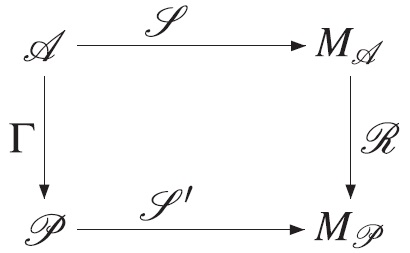
\includegraphics[width=100pt]{equivalance.jpg}
	\caption{The Transformation Soundness.}
	\label{ts}
\end{figure}





\begin{mydef}[Strong bi-simulation Relation]\label{strongb} A strong probabilistic
bi-simulation between two DTMCs $M_{1}$ and $M_{2}$ is a binary relation $\mathscr{R}$ iff whenever $s_{1}\mathscr{R}s_{2}$:

\begin{itemize}
	\item Each initial state of $M_{1}$ is related to at least one initial state $M_{2}$. 
			
	\item For each pair of states $s_{1}\mathscr{R}s_{2}$ and each transition  $s_{1} \rightarrow_{p_{1}} s_{1}'$ of either $M_{1}$ or $M_{2}$ there exists a transition $s_{2} \rightarrow_{p_{2}} s_{2}'$ of either $M_{1}$ or $M_{2}$, such that $p_{1} = p_{2}$.
    
\end{itemize}

\end{mydef}
For our proof, we stipulate herein the mapping relation $\mathscr{R}$ denoted by $M_{\mathscr{A}}\mathscr{R}M_{\mathscr{P}}$ between a DAC term $\mathscr{A}$ and its corresponding PRISM term $\mathscr{P}$.

\begin{mydef}[Mapping relation]\label{mappingR}  The relation $M_{\mathscr{A}}\mathscr{R}M_{\mathscr{P}}$  between a DAC term $\mathscr{A}$ and a PRISM term $\mathscr{P}$ such that $\Gamma(\mathscr{A})= \mathscr{P}$ is a strong bi-simulation relation.
\end{mydef}

Finally, proving that $\Gamma$ is sound means showing the existence of a strong bi-simulation between $M_{\mathscr{A}}$ and $M_{\mathscr{P}}$.

\newtheorem*{lem}{Lemma}
\begin{lem} [Soundness] The mapping algorithm $\Gamma$ is sound, \textsl{i.e.} $M_{\mathscr{A}}\sim M_{\mathscr{P}}$.\end{lem}

%%%%%%%%%%%%%%%%%%%%%
%\renewcommand{\qedsymbol}{}
%%%%%%%%%%%%%%%%%%%%%

\begin{proof} We prove $M_{\mathscr{A}}\sim M_{\mathscr{P}}$ by following a structural induction on DAC terms and their related PRISM terms. For that, let $s_{1}, s_{1}' \in \mathscr{S}_{A}$ and $s_{2}, s_{2}' \in \mathscr{S}_{P}$. We distinguish the following cases where L(s) takes different values: 


\begin{enumerate}
\item L($s_{1}$) = $\emph{l} : \overline{x}  \rightarrowtail \mathcal{N} $ such as $x=\left\{\emph{i},\emph{a}\right\} \Longrightarrow \exists s_{1} \rightarrow s_{1}'$, L($s_{1}$')= $l : x \rightarrowtail \overline{\mathcal{N}}$. For L($s_{2}$) = $\Gamma$(L($s_{1}$)), we have L($s_{2}$)=$ \left\langle L(x) ,\neg L(\mathcal{N}) \right\rangle$ then $\exists s_{2} \rightarrow s_{2}'$ where $L(s_{2}') = \left\langle \neg L(x), L(\mathcal{N})\right\rangle$.
	
\item  L($s_{1}$) = $\emph{l} : \overline{x}  \rightarrowtail \mathcal{N} $ such as $x=\left\{\emph{a!v},\emph{a?v}\right\} \Longrightarrow \exists s_{1} \rightarrow s_{1}'$, L($s_{1}$')= $l : x \rightarrowtail \overline{\mathcal{N}}$. For L($s_{2}$) = $\Gamma$(L($s_{1}$)), we have L($s_{2}$)=$ \left\langle L(x) ,\neg L(\mathcal{N}) \right\rangle$ then $\exists s_{2} \rightarrow s_{2}'$ where $L(s_{2}') = \left\langle \neg L(x), L(\mathcal{N})\right\rangle$.
	
\item L($s_{1}$) = $ \emph{l}: \overline{Ex(p,\mathcal{N}_{1}, \mathcal{N}_{2} )} $ then $\exists s_{1} \rightarrow_{p_{1}} s_{1}'$, L($s_{1}$')= $\emph{l}:Ex(p,\mathcal{N}_{1}, \overline{\mathcal{N}_{2}} )$. For L($s_{2}$) = $\Gamma$(L($s_{1}$)), we have L($s_{2}$)=$ \left\langle \emph{l} ,\neg l_{\mathcal{N}_{1}} ,\neg l_{\mathcal{N}_{2}} \right\rangle$ then $\exists s_{2} \rightarrow_{p_{2}} s_{2}'$ where $L(s_{2}') = \left\langle \neg\emph{l} ,l_{\mathcal{N}_{1}} ,\neg l_{\mathcal{N}_{2}} \right\rangle$.
    
    
\item  L($s_{1}$) = $ \emph{l}:\overline{D(g_{1},\mathcal{N}_{1}, \mathcal{N}_{2})}^{n}$ then $\exists s_{1} \xrightarrow{g_{1}}_{1} s_{1}'$, L($s_{1}$')= $\emph{l}:\overline{D(g_{1},\overline{\mathcal{N}_{1}}, \mathcal{N}_{2})}^{n-1}$. For L($s_{2}$) = $\Gamma$(L($s_{1}$)), we have L($s_{2}$)=$ \left\langle \emph{l} ,\neg l_{\mathcal{N}_{1}} ,\neg l_{\mathcal{N}_{2}} \right\rangle$ then $\exists s_{2} \xrightarrow{g_{1}}_{1} s_{2}'$ where $L(s_{2}') = \left\langle \neg\emph{l} ,l_{\mathcal{N}_{1}} ,\neg l_{\mathcal{N}_{2}} \right\rangle$.
	
\item L($s_{1}$) = $\emph{l} : \overline{\odot} $ then $\exists s_{1} \rightarrow_{1} s_{1}'$, L($s_{1}$')= $l :\odot$. For L($s_{2}$) = $\Gamma$(L($s_{1}$)), we have L($s_{2}$)=$ \left\langle \emph{l} \right\rangle$ then $\exists s_{2} \rightarrow_{1} s_{2}'$ where $ \forall \emph{l}_{i} \in \mathcal{L}$ : $L(s_{2}') = \left\langle \neg l_{i}\right\rangle$.
	
\item L($s_{1}$) = $\emph{l} : \overline{\otimes} $ then $\exists s_{1} \rightarrow_{1} s_{1}'$, L($s_{1}$')= $l :\otimes$. For L($s_{2}$) = $\Gamma$(L($s_{1}$)), we have L($s_{2}$)=$ \left\langle \emph{l} \right\rangle$ then $\exists s_{2} \rightarrow_{1} s_{2}'$ where $L(s_{2}') = \left\langle \neg l\right\rangle$.
	
\end{enumerate}




From the obtained results, we found that $p_{1}=p_{2}= 1$  in case 1, 2, 4, 5, 6 and $p_{1}=p_{2}= p,  0<p<1$ in case 3  means   $s_{1} \sim s_{2} $. In addition, the unique initial state of $M_{\mathscr{A}}$ is always corresponding to the unique initial state in $M_{\mathscr{P}}$. By studying all DAC terms, we find that $M_{\mathscr{A}}\sim M_{\mathscr{P}}$, which confirms that Lemma holds.\\

\end{proof}

In the following, we show that the mapping relation preserves the satisfiability of PCTL properties. This means, if a PCTL property is satisfied in the resulting model by a mapped function $\Gamma$ then it is satisfied by the original one.\\

\newtheorem*{prop}{Proposition}
\begin{prop} [PCTL preservation] For two DTMCs $M_{\mathscr{A}}$ and $M_{\mathscr{P}}$ such that $\Gamma(\mathscr{A})= \mathscr{P}$ where $M_{\mathscr{A}}\sim M_{\mathscr{P}}$. For a PCTL property $\phi$, then: $(M_{\mathscr{A}} \vDash \phi) \Longleftrightarrow (M_{\mathscr{P}} \vDash \phi)$.\\
\end{prop}

\begin{proof}

The preservation of PCTL properties is proved by induction on the PCTL structure and its semantics. Since $M_{\mathscr{A}}\sim M_{\mathscr{P}}$ and by relying to the semantics of each PCTL operator $\zeta \in \{\cup, \cup^{\leq k}\} $, we find that $(M_{\mathscr{A}} \vDash \zeta) \Longleftrightarrow (M_{\mathscr{P}} \vDash \zeta)$ which means: $(M_{\mathscr{A}} \vDash \phi) \Longleftrightarrow (M_{\mathscr{P}} \vDash \phi)$ 
\end{proof}

\section{Implementation and experimental results}
\label{section8}
In order to implement our methodology for deployment-space-exploration, an Eclipse plug-in has been developed. The graphical tool used for creating SysML/MARTE models is Eclipse TopCased \footnote{http://www.topcased.org Toolkit in OPen source for Critical Applications \& SystEms Development.}. After the generation of the corresponding XML file of the main design, The plug-in parses the document and generates PRISM code for each Activity diagram in DTMC model in order to check the configuration against the PCTL property. Finally, the plug-in returns a message for the close-candidate that satisfy our reliability requirement. 
Our approach is illustrated on the case study of an embedded automotive control system designed according to \citep{Meedeniya2011835}. The objective of the optimization is to maximize the reliability of system (Section \ref{DeploymentQualityMeasure}). To assess the performance of model checking on automotive systems, two software components are deployed on dedicated hardware architecture namely the Anti-lock Brake System (ABS) and Adaptive Cruise Control (ACC). It is assumed in our analysis that the information exchange among the components does not generate any information anomalies or abnormal signal transmission. However, the main anomalies come from the processors failures according to our assumptions in the beginning. When the failure occurs, an exception node is activated to restart the block behavior activity. In our specification the physical platform is depicted in Fig.\ref{hardplatform}. Table.\ref{swparam} refers to software components parameters.


\textbf{Hardware Architecture}: The hardware architecture used for the case study consists of four processors and three buses connecting the processors together as shown previously in Section \ref{section3}- Fig.\ref{hardplatform} abstracted in Fig.\ref{topo}. Table.\ref{parameters1} contains the parameters of processors (PR). 

\begin{table}
	\begin{center}
		
		\begin{tabular}{ l   c   c }
			
			\hline
Hardware &  \emph{Processing Speed}[MIPS]  & \emph{Failure Rate} \\ 
			\hline
PR 0 & 20                 & 9.10$^{-6}$       \\
PR 1 & 5                   & 2.10$^{-6}$           \\				
PR 2 &  5                   & 3.10$^{-6}$   \\
PR 3 &  10                & 9.10$^{-6}$  \\		   			
			\hline	
		\end{tabular}
		\normalsize
	\end{center}
	\caption{Parameters of processors}
	\label{parameters1}
\end{table}







\begin{figure}[!htb]
	\centering

		\centering
		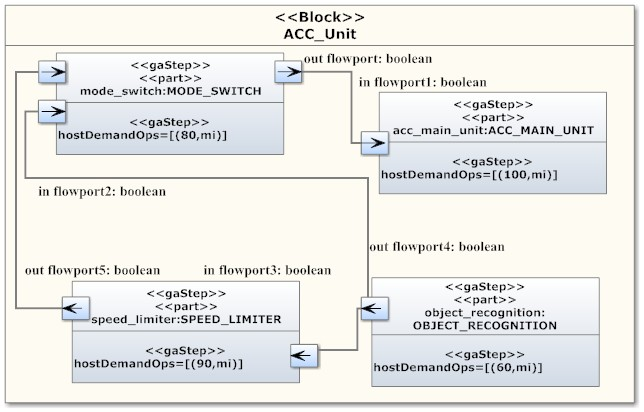
\includegraphics[width=250pt]{SwPlatformACC.jpg}
		\caption{Adaptive Cruise Control  }
		\label{comp1}

\end{figure}

\begin{figure}[!htb]
    \centering
    
    \centering
    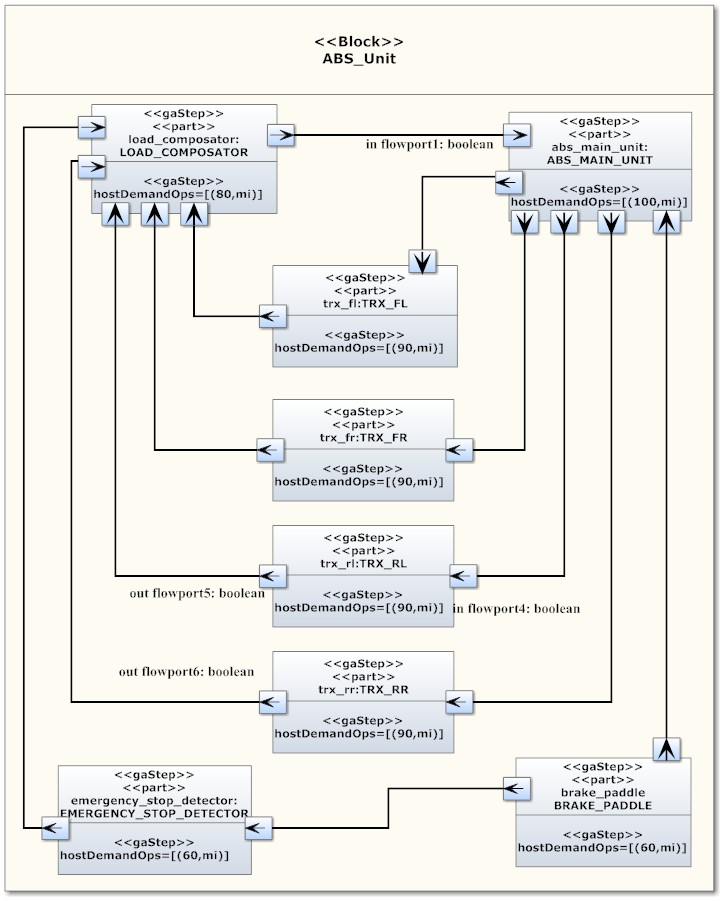
\includegraphics[width=350pt]{SwPlatformABS.jpg}
    \caption{Anti-lock Brake System  }
    \label{comp2}
    
\end{figure}

\begin{figure}[!htb]
	\centering
	\begin{minipage}{.5\textwidth}
		\centering
	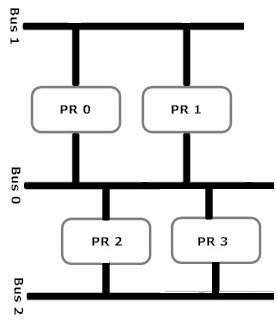
\includegraphics[width=150pt, height=150pt]{hardwareTopology.jpg}
	\caption{Hardware topology}
	\label{topo}
	\end{minipage}%
	\begin{minipage}{0.5\textwidth}
		\centering
	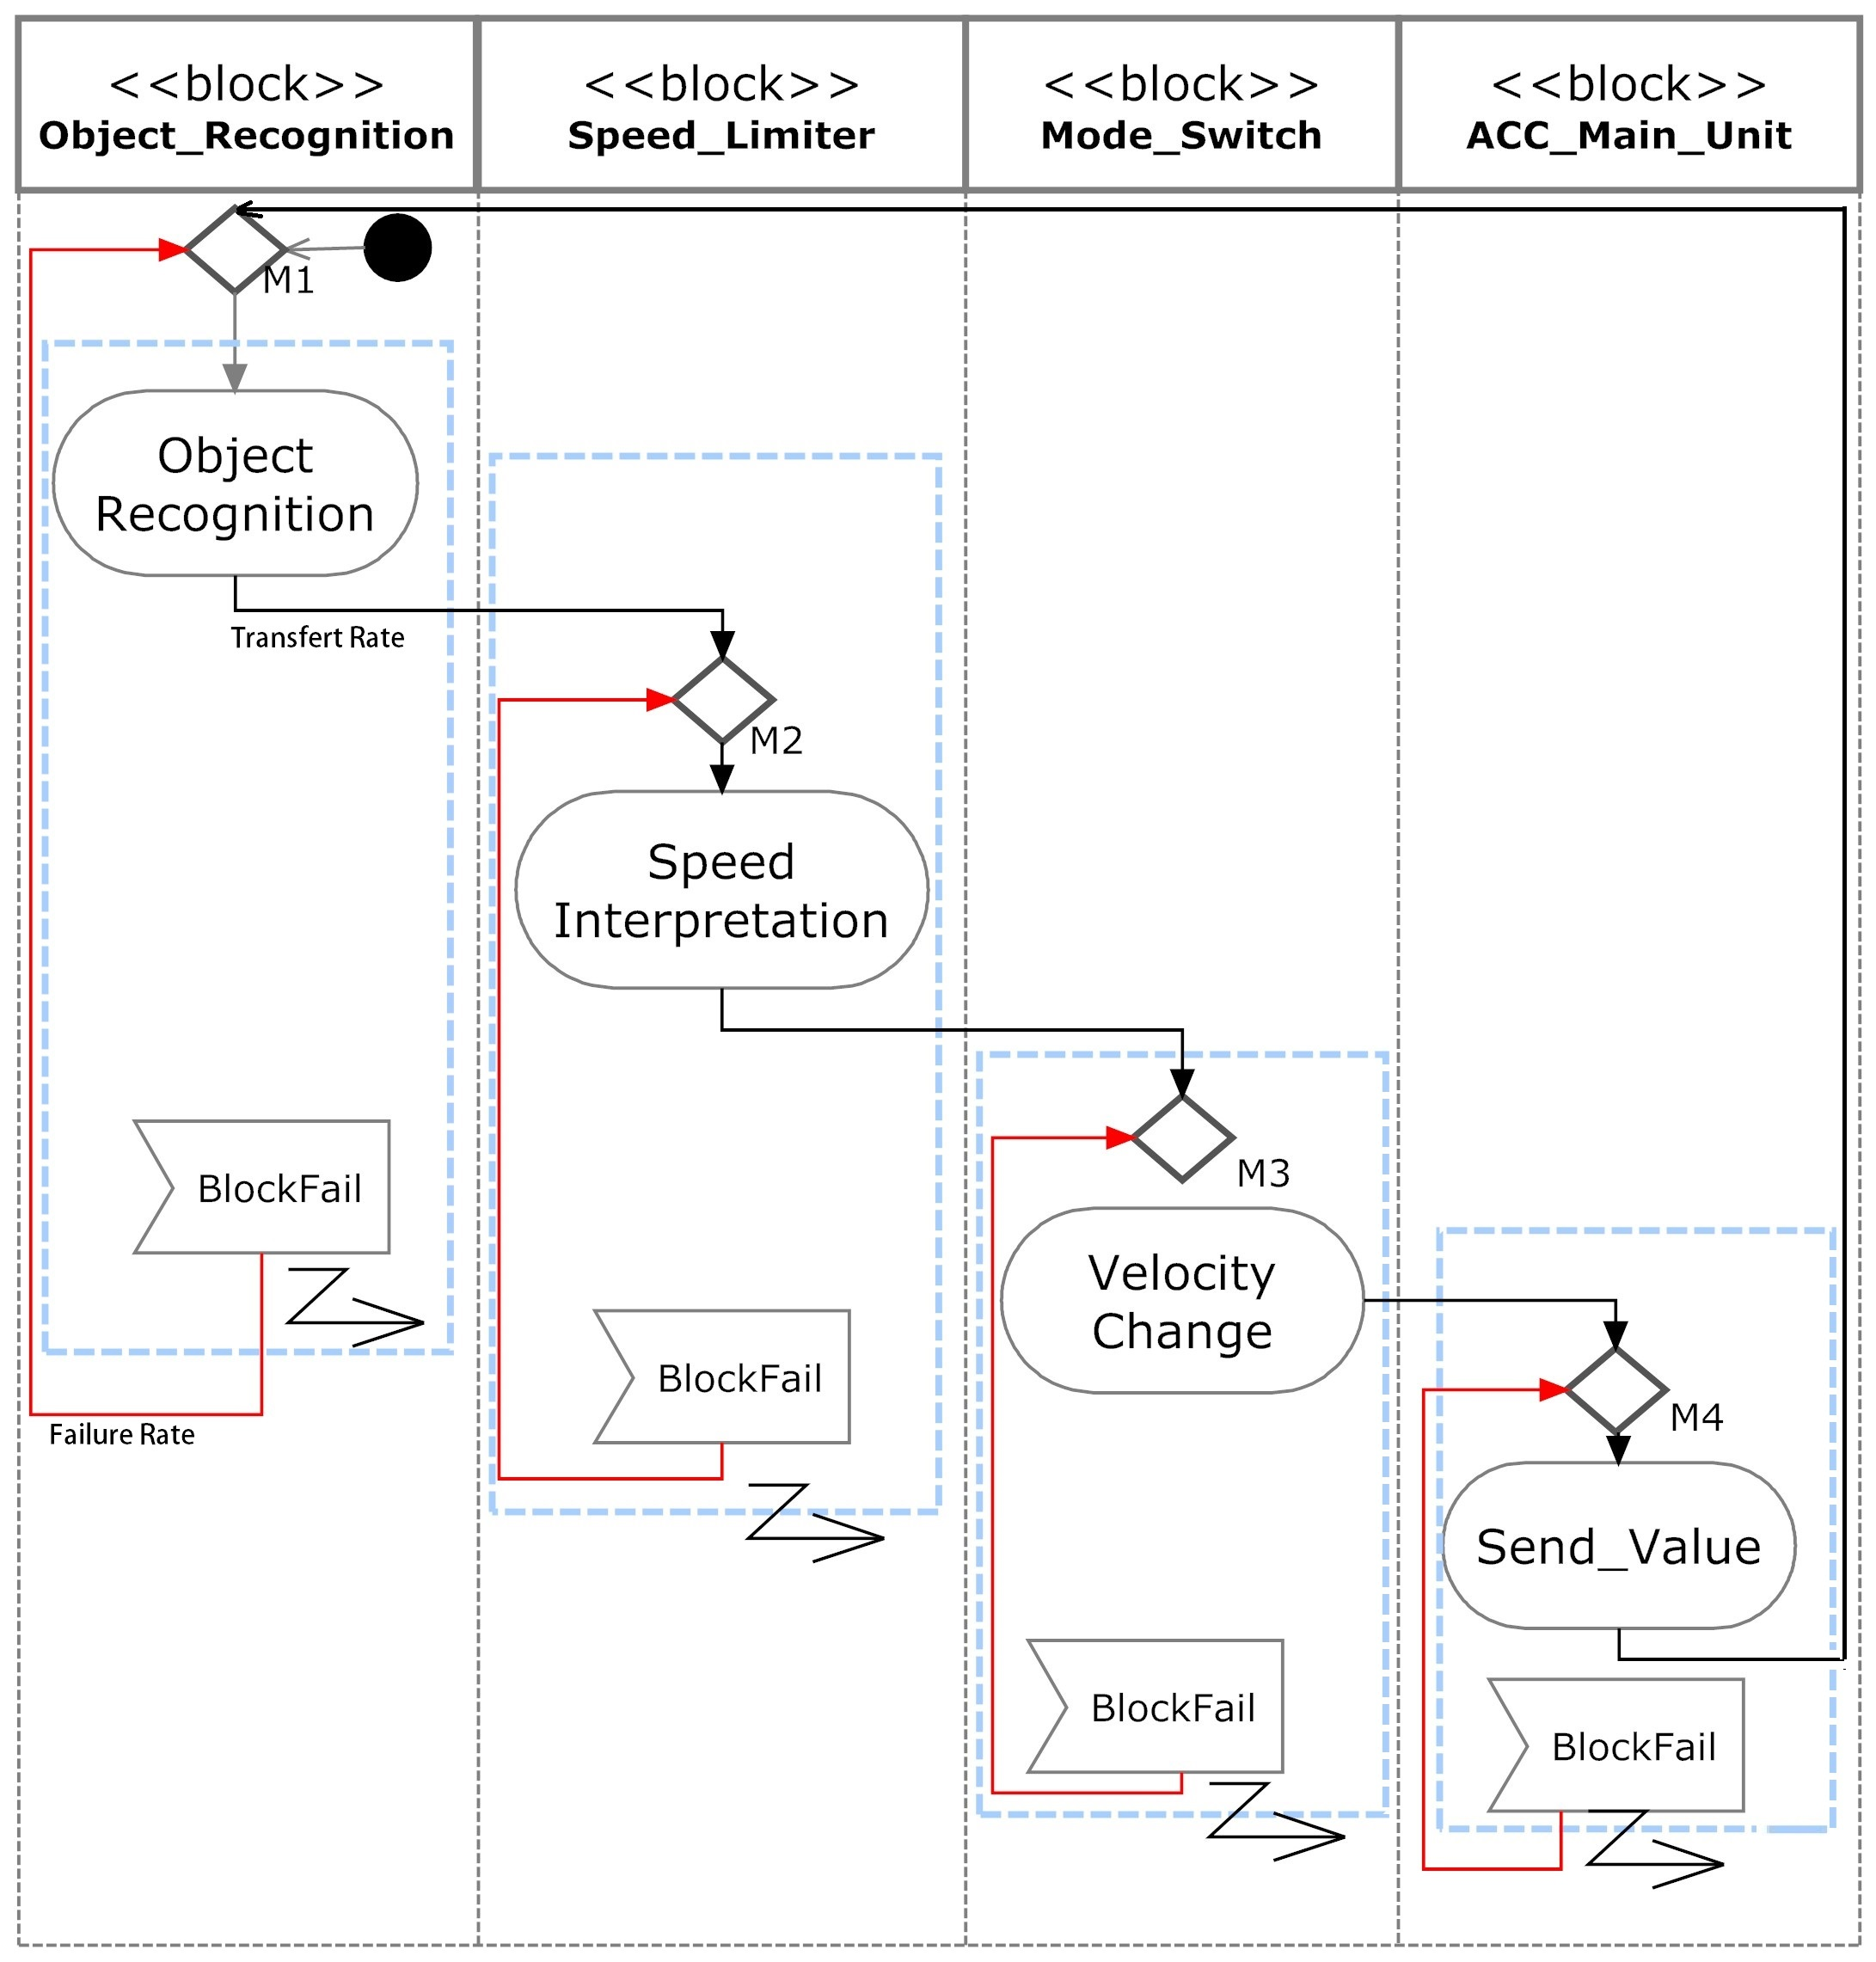
\includegraphics[width=200pt]{ActivityACC.jpg}
	\caption{Activity diagram for Adaptive Cruise Control}
	\label{acc1}
	\end{minipage}
\end{figure}




\begin{figure}[!htb]
	\centering
	
	\centering
	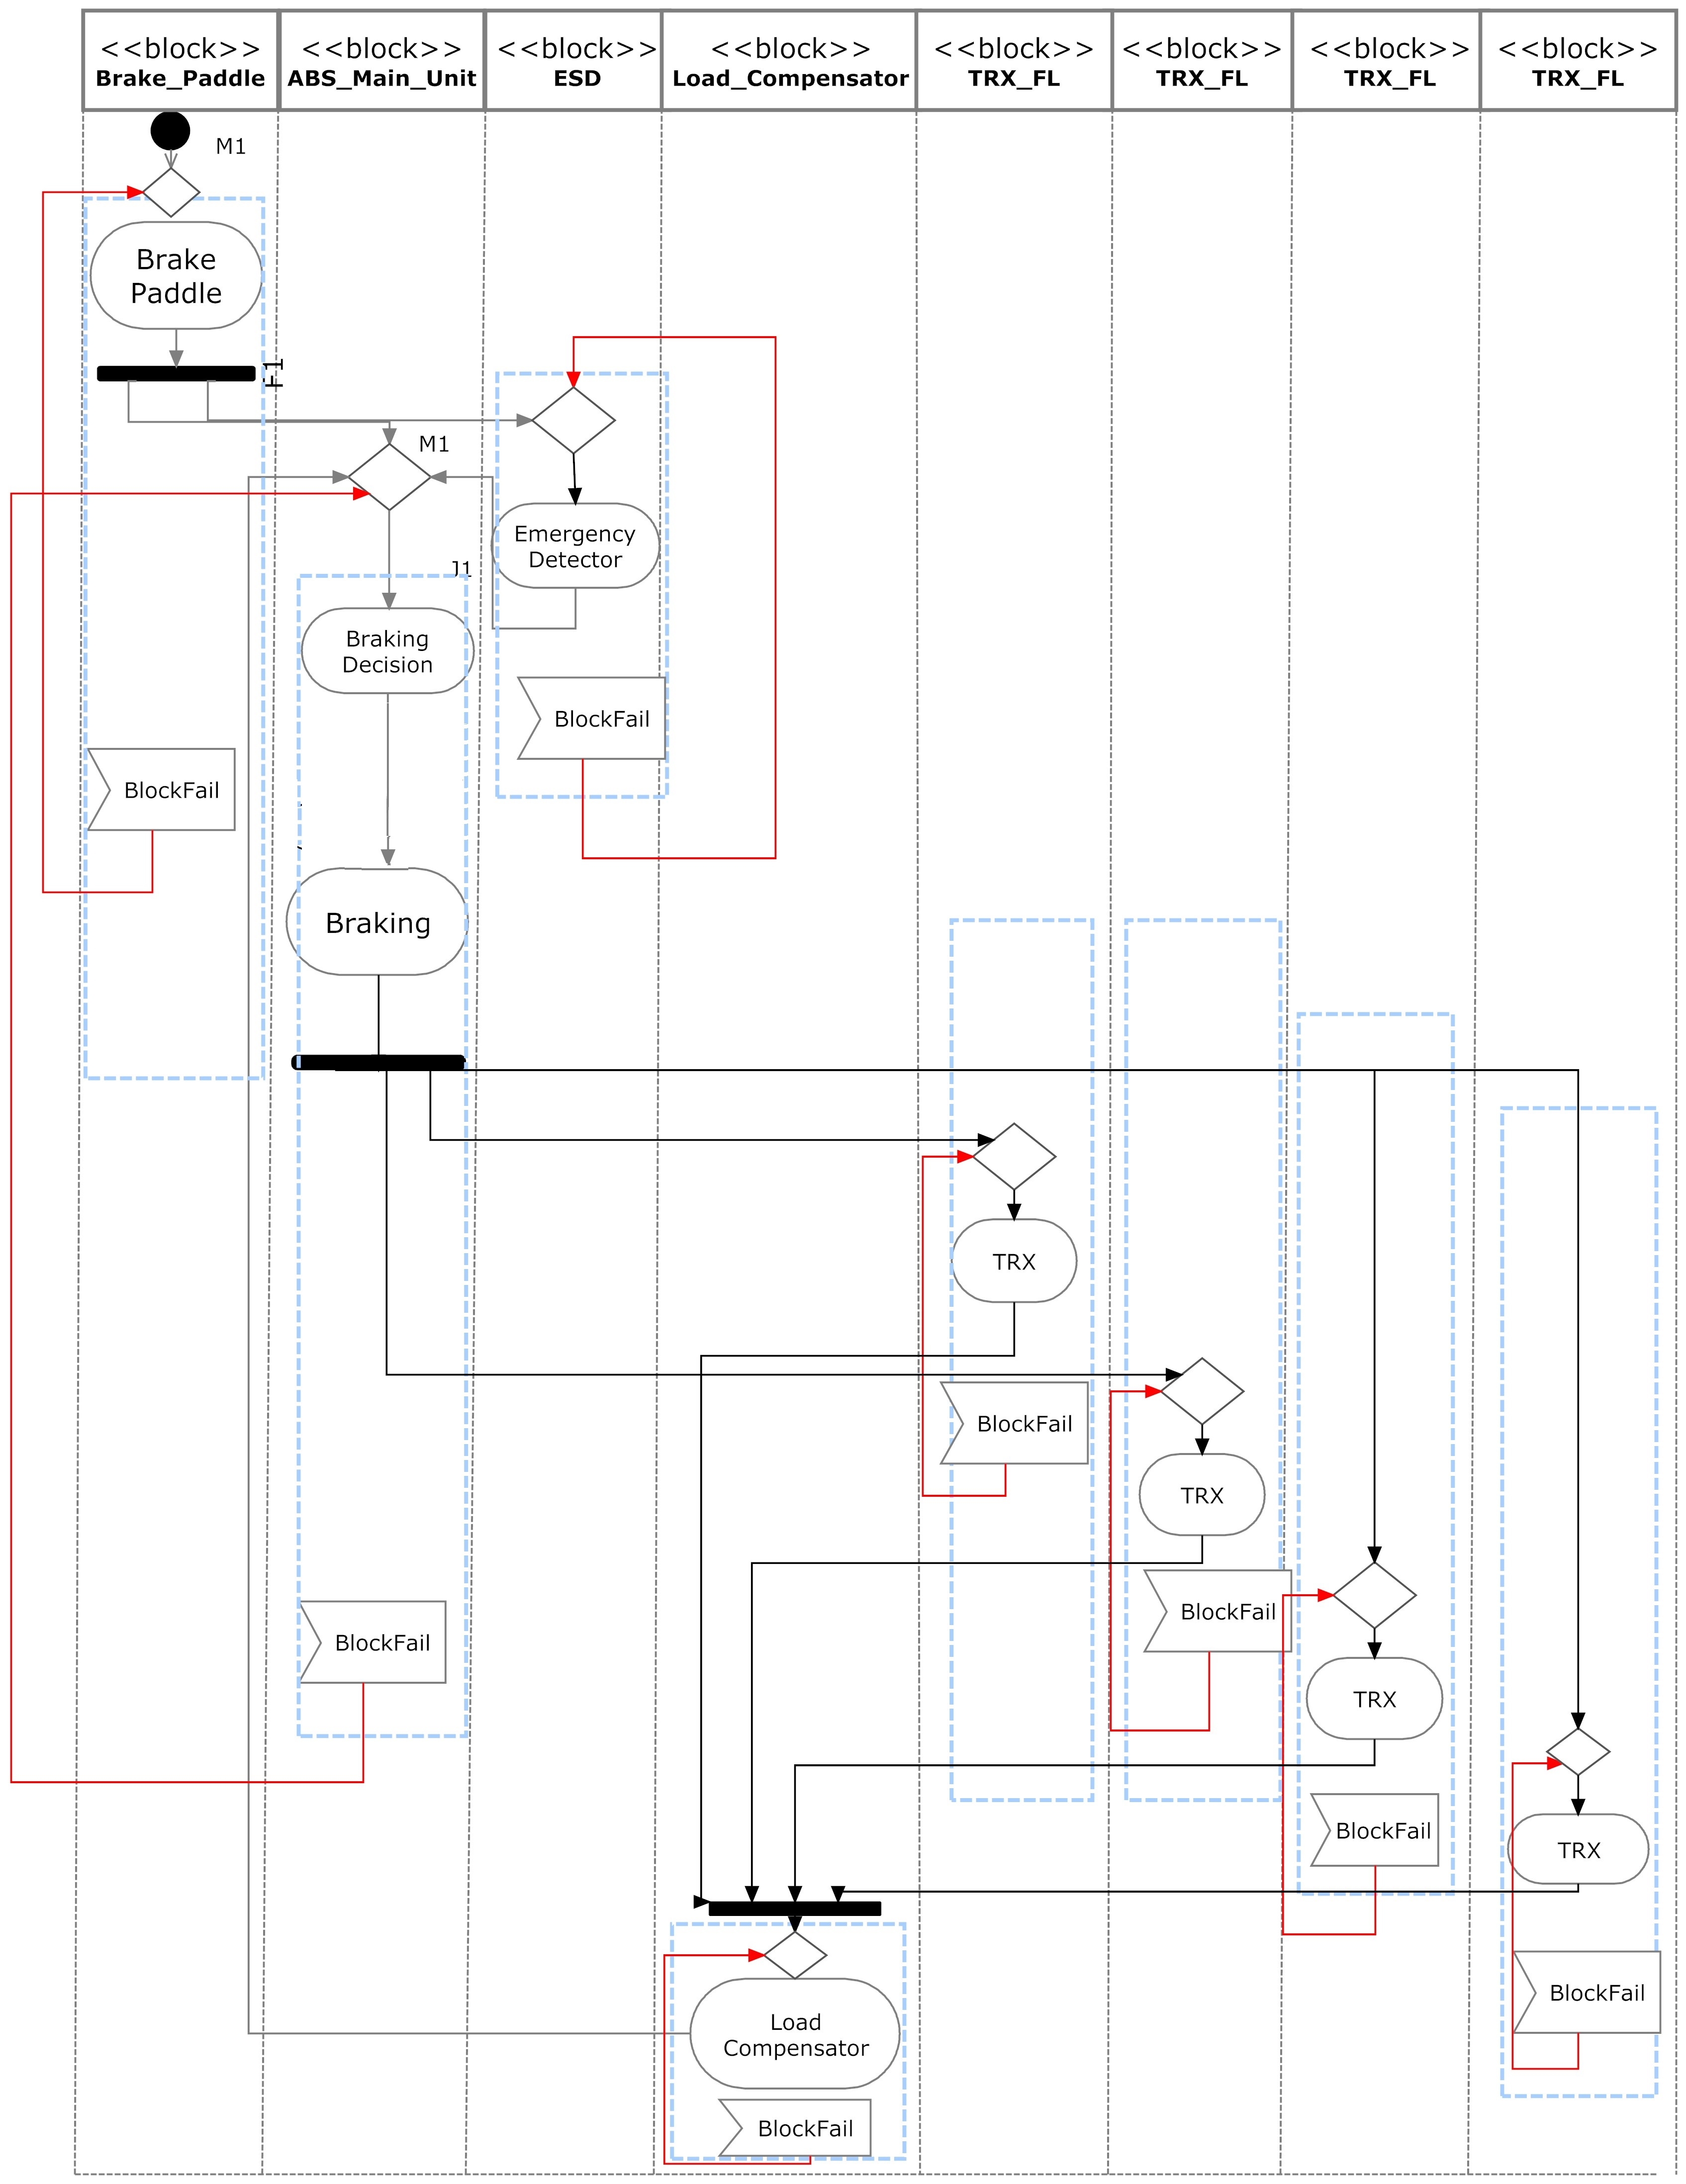
\includegraphics[width=350pt, height=340pt]{ActivityAbs.jpg}
	\caption{Activity diagram for Anti-lock Brake System }
	\label{abs1}
	
\end{figure}




\textbf{Anti-lock Brake System (ABS)}: used in modern cars to minimize hazards associated with skidding and loss of control due to locked wheel during braking. The software architecture of the ABS is depicted in Fig.\ref{comp2} and Fig.\ref{abs1}(Associated Activity diagram) (components 0-7 in Table.\ref{swparam}). The ABS Main unit is the major decision unit regarding the braking levels for individual wheels, while Load Compensator unit assists with computing adjustment factors from wheel load sensor inputs. Component 4-7 (Table.\ref{swparam}) represent transceiver software components associated with each wheel, and communicate with sensors and brake actuators. \emph{Brake Paddle} is the software component that reads from the \emph{Paddle Sensor} and sends event to the emergency stop detection software module. 
 



\begin{table}[!htb]
	
	\begin{minipage}{.5\linewidth}
		
		\centering
		
	\begin{tabular}{ l l  c }
		
		\hline
		\emph{i }& \emph{SW component }&  \emph{wl}(c$_{i}$)[KB] \\ 
		\hline
		0 & ABS\_MAIN\_UNIT& 60 \\
		1 & EMERGENCY\_STOP\_DETECTOR& 90 \\
		2 & BRAKE\_PADDLE& 150 \\
		3 & LOAD\_COMPENSATOR& 100 \\
		4 & TRX\_RR& 90 \\	
		5 & TRX\_RL& 60 \\
		6 & TRX\_FR& 90 \\
		7 & TRX\_FL& 150 \\
		8 & ACC\_MAIN\_UNIT& 100 \\
		9 & MODE\_SWITCH& 90 \\		
		10 & OBJECT\_RECOGNITION& 60 \\
		11 & SPEED\_LIMITER& 90 \\					
		\hline	
	\end{tabular}
	\caption{Software components parameters}
	\label{swparam}
		
	\end{minipage}%
	\begin{minipage}{.6\linewidth}
		\centering
		
		
			\begin{tabular}{ l m{3cm} }
				
				\hline
				Hardware &  Components \\ 
				\hline
			PR 0 & 4,11,9,7\\
            PR 1 & 2,5,1\\				
            PR 2 & 3,6,0\\
            PR 3 & 8,10\\
				
				\hline	
			\end{tabular}
			\normalsize
			
			\caption{Allocation results}
			\label{topoc}
		
		
		
		
	\end{minipage} 
\end{table}



\textbf{Adaptive Cruise Control (ACC)}: The aim of this component is to avoid crashes by reducing speed once the slower vehicle in front is detected. The main software components used by ACC are depicted in Fig.\ref{comp1}  and Fig.\ref{acc1}(Associated Activity diagram). Service initialization is possible at Object Recognition software that communicate with sensors. Speed Limit, Mode Switch and Brake Paddle contribute to triggering of the service. The captured data are processed by the ACC\_MAIN\_UNIT and Human Machine Interface to communicate with actuators. 


  	\lstset{
  		basicstyle=\ttfamily\scriptsize,
  		numbers=left,
  		numberstyle=\scriptsize,
  		numbersep=3pt,
  		caption=ACC PRISM code fragment,
  		frame=single,
  		captionpos=b,
  		label=sourcecode,
  		tabsize=2,
           linewidth=14.5cm
  	}
  	\tiny
  	
  	
  	\begin{table}[!ht]

  			\begin{center}


  			\begin{tabular}{ p{14.5cm} }
  	\begin{lstlisting}
dtmc

const double P1;
const double P2;
const double P3;
const double P4;
module ACC
Initial : bool init true;
Object_Recognition: bool init false;
Speed_Interprestation:bool init false;
Velocity_Change : bool init false;
Send_Value : bool init false;
Final: bool init false;

Proc_Fail: bool init false; 
.........

D1: bool init false;
D2: bool init false;
...........

M11: bool init false;
M12: bool init false;		
M1: bool init false;		
[Initial] Initial -> (Initial'=false)&(M11'=true);
[M11]M11 -> (M11'=false)&(M1'=true);		
[M12]M12 -> (M12'=false)&(M1'=true);		
[M1]M1 -> (M1'=false)&(Object_Recognition'=true);		
[Object_Recognition] Object_Recognition -> 1.0:(D1'=true)&
(Object_Recognition'=false);

[D1] D1 -> P1:(M21'=true)& (D1'=false)+(1-P1):(Block1_Fail'=true)&(D1'=false);
[Block1_Fail] Block1_Fail-> (Block1_Fail'=false)& (M12'=true);		
[Speed_Interpretation]Speed_Interpretation -> 1.0:(SpeedInterprestation'=false)
&(D2'=true);		
[D2] D2 -> P2:(M31'=true)& (D2'=false)+(1-P2):(Block2_Fail'=true)&(D2'=false);
[Block2_Fail] Block2_Fail-> (Block2_Fail'=false)& (M22'=true);	
[Velocity_Change] Velocity_Change -> 1.0:(Velocity_Change'=false)&
(D3'=true);		
[D3] D3 -> P3:(M41'=true)& (D3'=false)+(1-P3):(Block3_Fail'=true)&(D3'=false);
[Block3_Fail] Block3_Fail-> (Block3_Fail'=false)& (M32'=true);	
[Send_Value] Send_Value -> 1.0:(Send_Value'=false)&(D4'=true);		
[D4] D4 -> P4:(Final'=true)& (D4'=false)+(1-P4):(Block3_Fail'=true)&(D4'=false);
[Block4_Fail] Block4_Fail-> (Block4_Fail'=false)& (M42'=true);		
endmodule 

label "ProcFail" = Block1_Fail|Block2_Fail|Block3_Fail|Block4_Fail; \end{lstlisting} 	


\\


\end{tabular}

            
                \end{center}
\end{table}
\normalsize
\subsection{Evaluation}

Despite the low number of components and states (i.e.PRISM states) generated after mapping, the deployment-space exploration took 1622 seconds which is approximately 27 minutes. Our plug-in records each result of checked model to get the minimum failure probability of each deployment candidate. During this process, 3256 candidates was explored and performed on i7 CPU 2.67GHz with 8.0GB of RAM. The listing.\ref{sourcecode} shows the PRISM code that can be parametrized through the double constants values. The constant values are filled with our plug-in during the deployment-space-exploration (i.e. Model checking process). 

Reliability property of ACC and ABS that we analyze using PRISM is :`` the probability that a ACC and ABS will need to be replaced by a new one after T time steps'' and expressed using PCTL property:
\begin{equation}
    P=? [true \cup ^{\leq T} (``Proc\_Fail'')] , T=200
\end{equation}





In the property above \emph{Proc_Fail } asserts that the processor is in failing state when one of the software blocks fail according to the PRISM \emph{label} :

\begin{equation} label ``Proc\_Fail" = Block1\_Fail | Block2\_Fail |Block3\_Fail |Block4\_Fail
\end{equation}


The analysis results of reliability property obtained from PRISM are as follows: The result of the property in case of ACC is shown in Fig.\ref{pr1}; the result of property in case of ABS is shown in Fig.\ref{pr2}. For better deployment; we choose the minimum probability in case of failure. In Table.\ref{topoc}, we show the best software blocks candidate relative to the probabilistic results. In the first figure (ACC), the failure occurs after 200 time steps with probability near to 0.542\% and could be deployed on two processors where the second figure (ABS), the failure occurs after 200 time steps with probability near to 0.579\% and could be deployed on three processors. The cases where the blocks deployed on one processor \emph{are not considered} in our approach.



\begin{figure}[!htb]
	\centering
	\begin{minipage}{.5\textwidth}
		\centering
		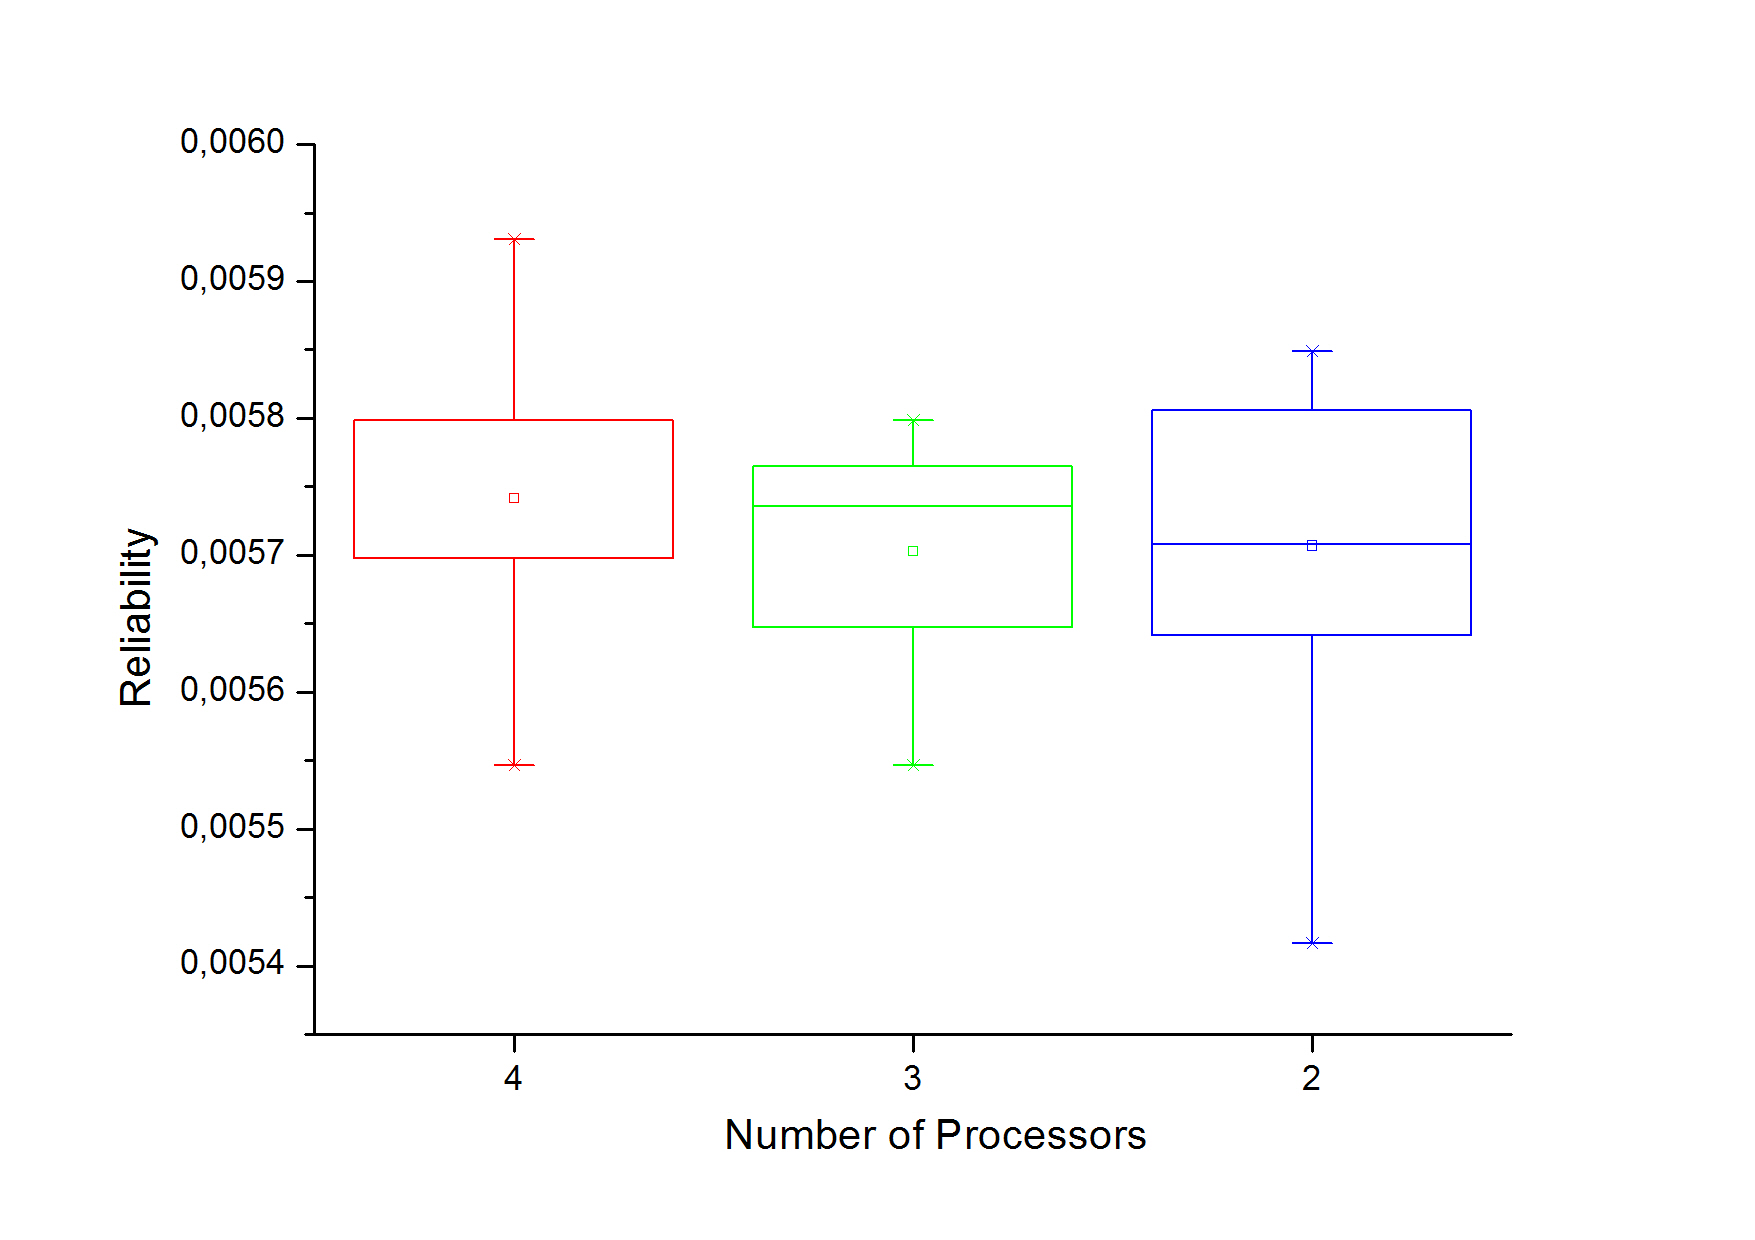
\includegraphics[width=180pt, height=135pt]{graph002.jpg}
		\caption{ACC Reliability}
		\label{pr1}
	\end{minipage}%
	\begin{minipage}{0.5\textwidth}
		\centering
		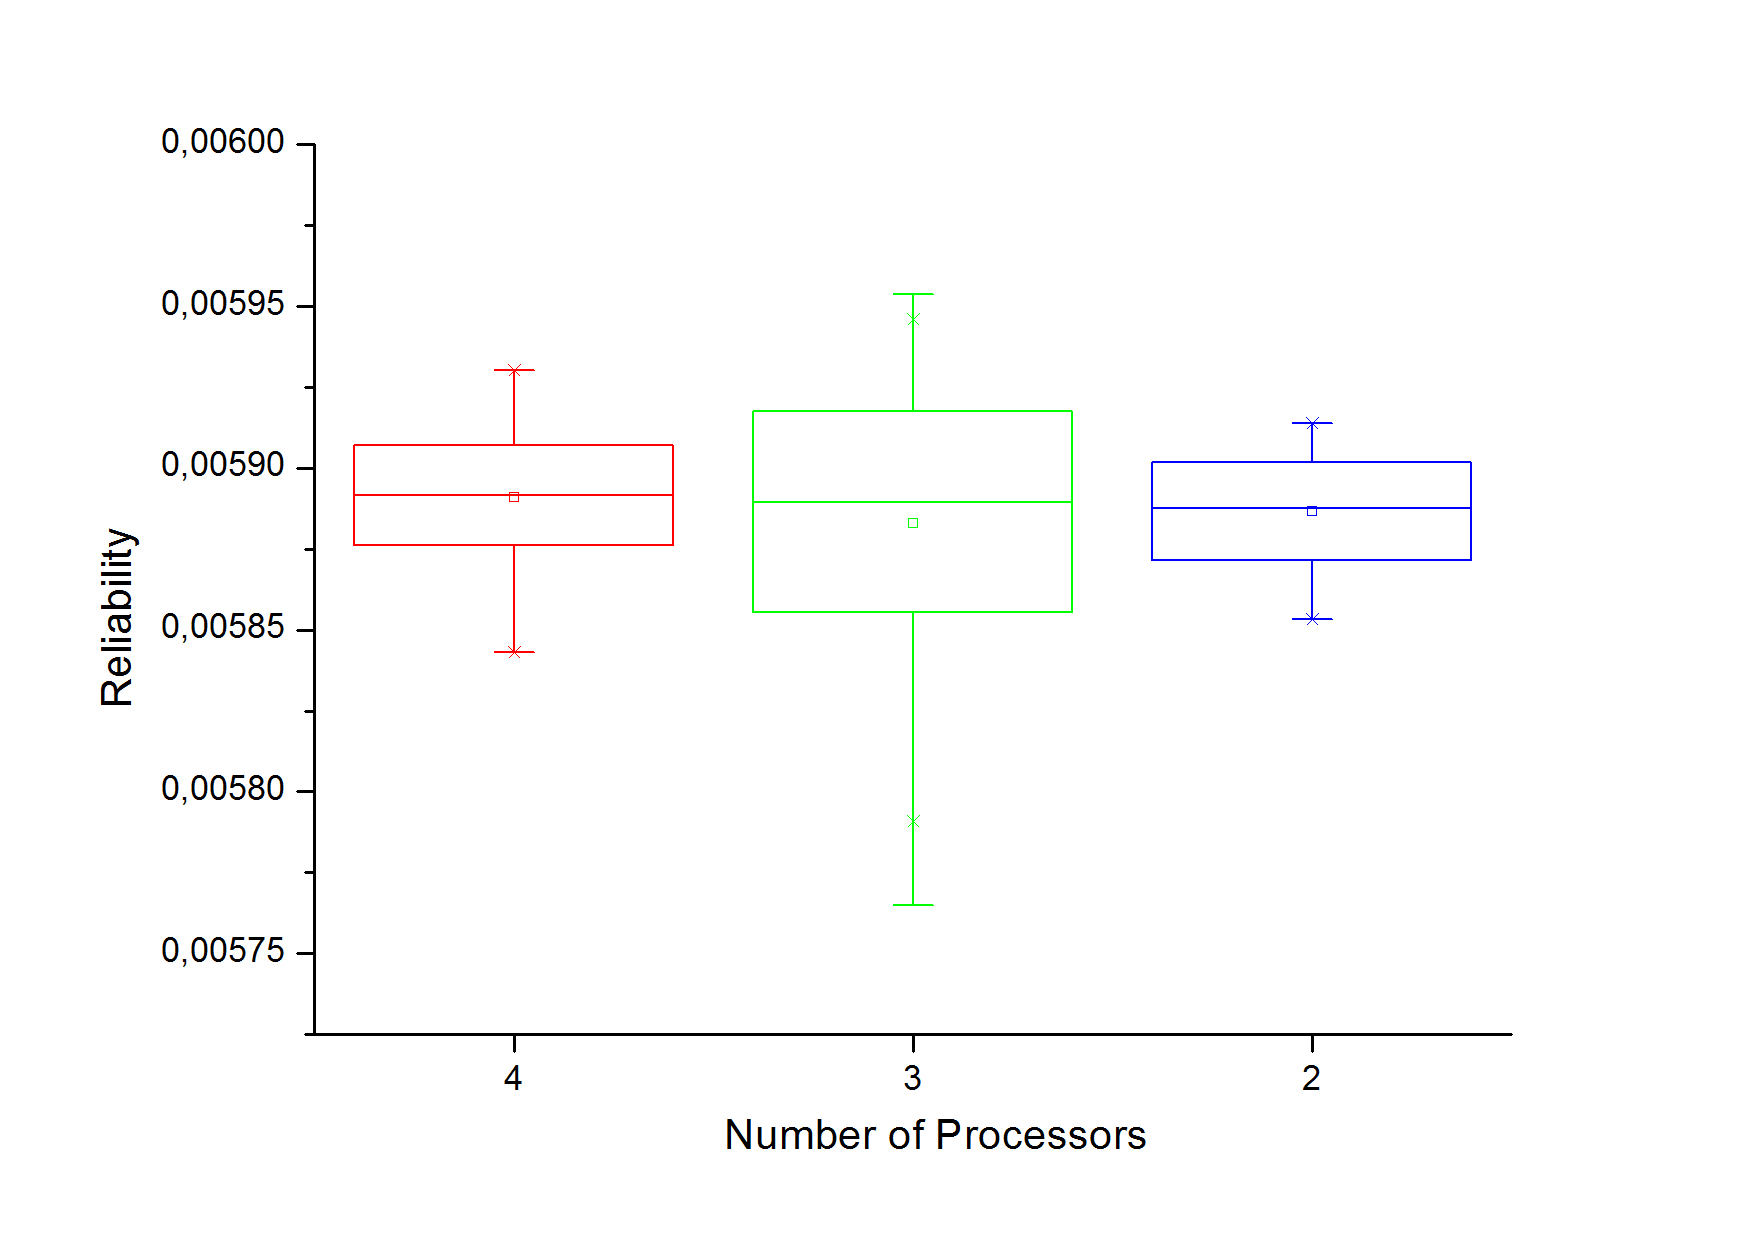
\includegraphics[width=180pt, height=135pt]{graph001.jpg}
		\caption{ABS Reliability}
		\label{pr2}
	\end{minipage}
\end{figure}  
  
\subsection{System constraints  and  optimization}

\begin{figure}[htbp]
    \centering
    \begin{subfigure}{.5\textwidth}
        \centering
        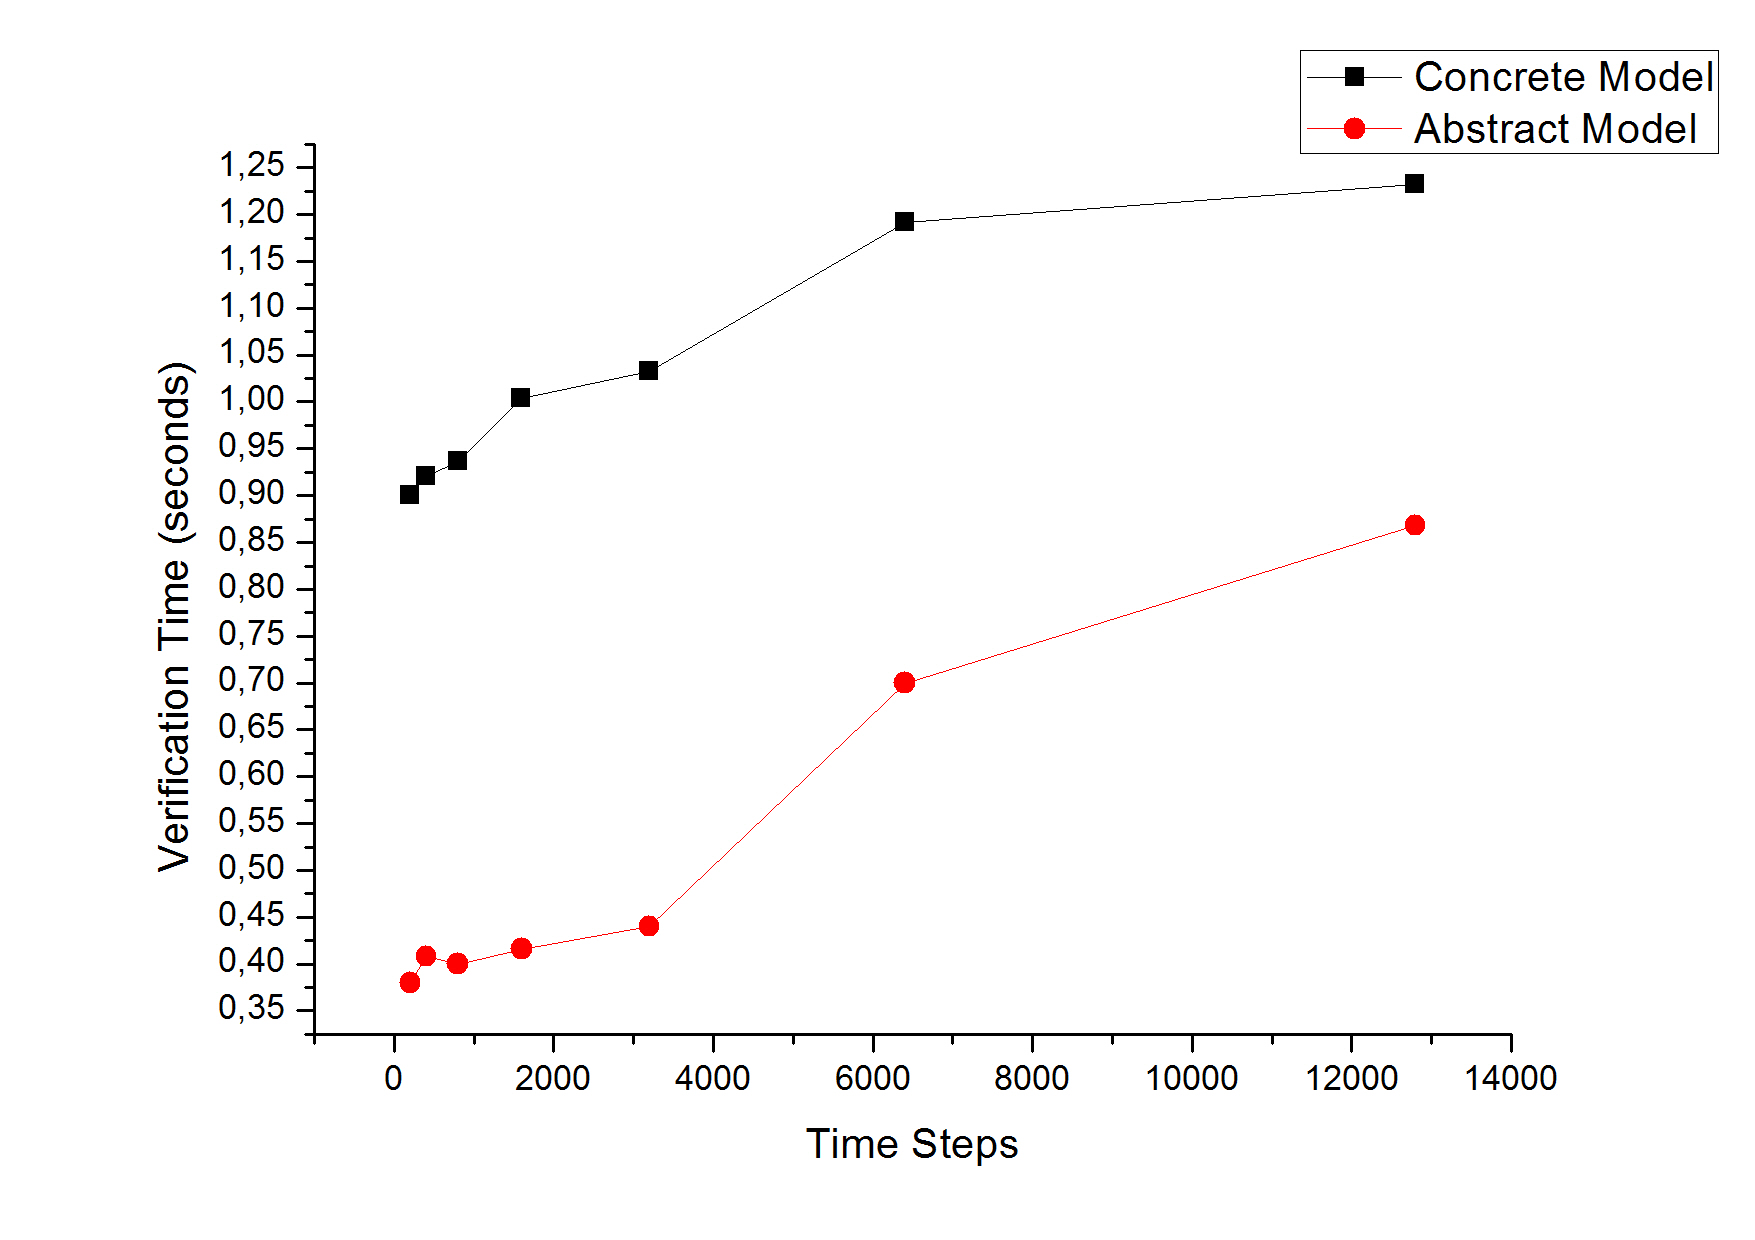
\includegraphics[width=180pt, height=135pt]{graph02.jpg}
        \caption{Verification Time}
        \label{fig02}
    \end{subfigure}%
    \begin{subfigure}{.5\textwidth}
        \centering
        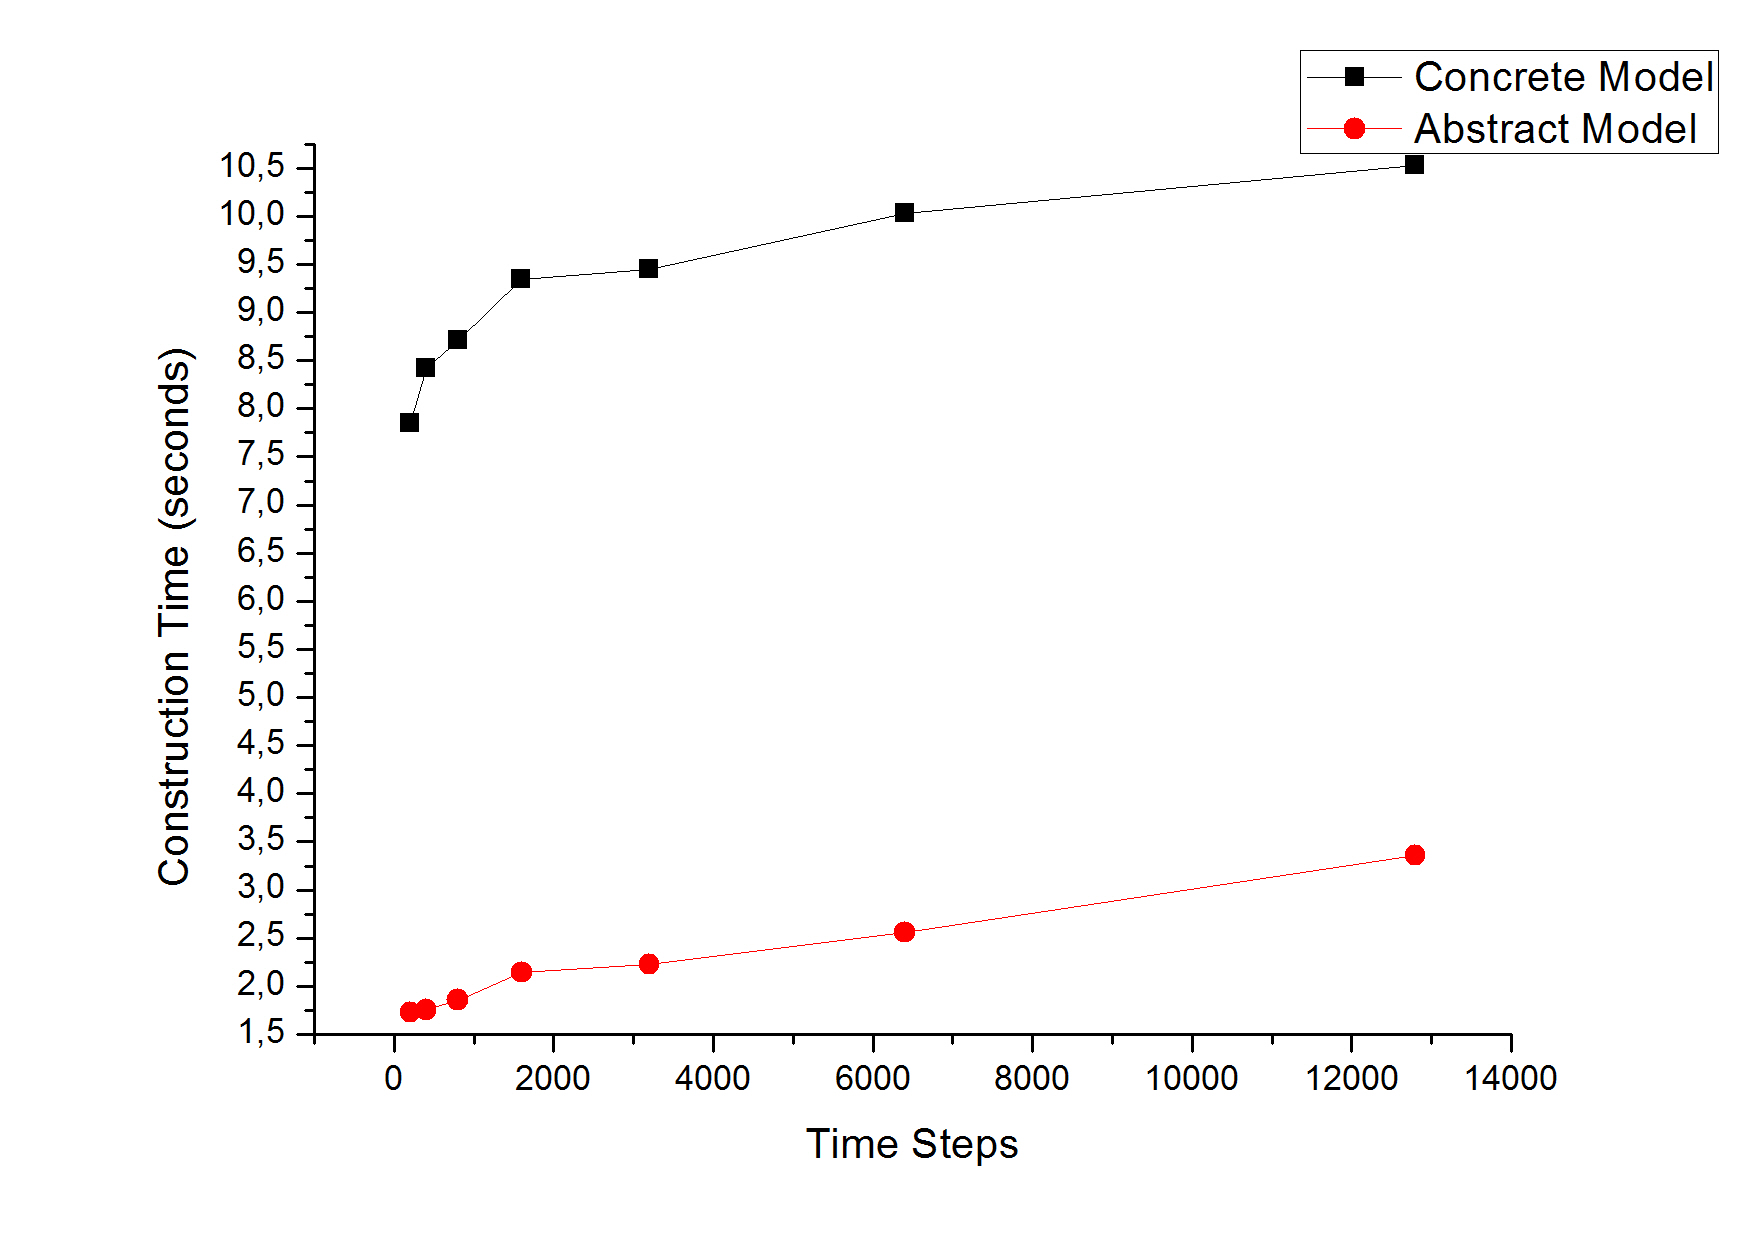
\includegraphics[width=180pt, height=135pt]{graph01.jpg}
        \caption{Construction Time}
        \label{fig01}
    \end{subfigure}
    \caption{The abstraction effects on ABS diagram}
    \label{figaabs}
\end{figure}





\begin{table}[!tp]
    \scriptsize	
    \begin{center}
        \begin{tabular}{  p{1.5cm}p{2cm}p{2cm}p{2cm}p{2cm}m{1.5cm}   }
            \hline
            \multirow{2}{1.5cm}{Time Steps} &\multicolumn{2}{c}{ Concrete Model} & \multicolumn{2}{c}{Abstract Model} &  \multirow{2}{1.5cm}{Results}  \\
           %\cline{2-5}
            & Tc & Tv & Tc & Tv& \\
            \hline
           200 & 7.844&0.900&1.728&0.380 &0.00579\\
            400  & 8.720&0.920&1.756&0.408&0.0169\\
            800 & 8.416&0.936&1.856&0.400&0.0233\\
            1600&9.348&1.004&2.144&0.416&0.0462\\
            3200&9.448&1.032&2.224&0.440&0.0905\\
            6400&10.036&1.192&2.560&0.800&0.1729\\
            12800&10.532&1.232&3.360&1.168&0.3160\\
            \hline
        \end{tabular}
        \caption{Abstraction results .}
        \label{tabaabs}
    \end{center}
\end{table}



In our experiment, we have accepted a few properties to make our model simple and applicable to larger system. The software failure are not considered and they are assumed independent to the deployment. All the deployment parameters could be obtained (e.g. Processor speed) except processors failing parameters. Failure parameters could be estimated by experts using profiling \citep{Houssin2014107}. 

One of the challenges in applying probabilistic model checking is \emph{scalability}: the models need to be constructed and analyzed are time consuming and affects the design-space exploration.  This phenomenon is called \emph{state-explosion problem}. 

For this purpose we apply the algorithm and rules defined by \citep{Ouchani2014} to observe the abstraction effects on SysML Activity diagram in Fig.\ref{abs1} with the best deployment candidate parameters values. The abstraction approach produce a reduced activity diagram without the irrelevant actions (i.e.unreachable actions) based on the PCTL property. The result is shown in Table.\ref{tabaabs} presents its different verification results in function of time steps T (i.e. Path length). To evaluate the verification cost, we measure the time required for model checking, denoted by Tv and time required to construct the model denoted by Tc.
The results are depicted in Fig.\ref{figaabs}. The number of states and transitions for the concrete model are 16461  states and 93412  transitions, respectively and 3025 states, 15491 transitions for the abstracted model. we notice that the abstraction rules preserves the results while verification and construction time are optimized.

In addition, PRISM model checker implements an interesting mechanism to handle the state explosion using binary decision diagrams \citep{KP12}. This engine enables probabilistic verification of models up to $10^{10}$ states. PRISM includes advanced techniques for model abstraction based on stochastic games \citep{Kwiatkowska2009}. It also supports approximate probabilistic model checking using statistical methods. So, with the capability of PRISM engine, it is possible to analyze larger systems using our methodology.

\section{Discussion and threats to validity}
\label{section9}


\subsection{Use of SysML}
Through the application of  our methodology, we found that SysML is an acceptable language in industrial contexts since it is a good fit for capturing behavioral and structural aspects of system in our study. Nevertheless, using SysML for complex design with accurate structural properties is not feasible. So, we found the extendability aspect of SysML language to be advantageous for system engineering. The designer can develop its proper profile to support a specific properties. In case of our methodology, we introduce MARTE profile as shown in Fig.\ref{hardplatform}. We found that profile very useful for specifying hardware and software  properties to perform our analysis.

\subsection{Architecture-level alternatives}
The main observation from the experimental results confirms our proposed idea based on the   parameterizable Markov model \citep{Filieri2016} has an impact on the system reliability. The proposed methodology explores all the architectural alternatives to select a suitable one that fulfills the reliability requirement expressed in temporal logic. The inputs parameters of each alternative is computed from the properties of our electronic automotive system. The overhead of such computation is negligible in our experiments since it occurred before the design space exploration.

\subsection{Threats to validity}
The approach discussed in this paper focuses on the reliability that is hardware-dependent.  The utility of the approach is to derive the optimal deployment candidate based on few relevant metrics discussed in the published paper \citep{Meedeniya2011835}.  To handle the automotive system failures, our approach expresses the system-services flow through activity diagram partitioned on  software components. We assume that the external environment  factors do not influence the system reliability. In addition, the problem of power and energy consumption still exists which limits the performance and reliability of our system. These issues deserve attention in our  future work.

\section{Conclusion}
\label{section10}


In this paper, we presented a deployment-exploration approach of embedded software modeled by using SysML internal blocks diagram. The first objective is to validate a deployment in case of hardware failures that generally emerge in system design-flow and secondly to reduce the cost of maintenance and repairing. The proposed approach use SysML blocks diagram with additional real time system annotations using MARTE profile where behavior is expressed using SysML Activity diagram. Compared to \citep{Meedeniya2011835} and \citep{Thiruvady20141937}, which use genetic algorithms, our approach leverages probabilistic modeling thus allowing the assessment of properties formally expressed in probabilistic temporal logic. With respect to \citep{Besnard201554} which use a scheduling algorithm for allocation in AADL, leads to a difficulty to obtain a good partitions due to the constraints limited to time, we employ a probabilistic formula based on reliability-relevant
attributes. Moreover, in contrast to \citep{Brosse2012}, which is based on code generated for performance estimation area and early power figures, our approach extracts the relevant information directly from the specification and maps the behavior to PRISM for model checking.    

The research contribution of this work consists on capturing the system behavior as Discrete-Time Markov chains (DTMC) supported by PRISM language. We proposed a calculus dedicated to flow observation on blocks behavior that captures precisely the underlying semantics. In addition, we formalized PRISM language and showing its semantics. Moreover, we proved the soundness of our proposed approach by defining the relation between the semantics of the mapped diagrams and the resulting PRISM models. By this relation, we proved the preservation of the satisfiability of PCTL properties. We have shown the effectiveness of our approach in realistic case study: Embedded automotive control system. 

The practical advantages of the proposed approach in the context of deployment, consists on providing key decision for the acceptable candidate via probabilistic model checking. In addition, the results of our approach using PRISM could be plotted as graphs to be inspected for interpretations and anomalies. 

The presented work can be extended in the following two directions. First, we intend to extend our approach to support more constraints that affect the entire system behavior such as energy, bus loads and memory restrictions. Finally, we intend to translate the system into specific language such as VHDL/C/C++/NesC for simulation. 



\bibliographystyle{plainnat}
\bibliography{biblatexbaouya}

%% Authors are advised to use a BibTeX database file for their reference list.plainnat
%% The provided style file elsarticle-num.bst formats references in the required Procedia style

%% For references without a BibTeX database:

% \begin{thebibliography}{00}

%% \bibitem must have the following form:
%%   \bibitem{key}...
%%

% \bibitem{}

% \end{thebibliography}

\end{document}

%%
%% End of file `ecrc-template.tex'. 